	%!TEX root = ../thesis.tex
%*******************************************************************************
%*********************************** Theory chapter *****************************
%*******************************************************************************

\chapter{Theory}

\graphicspath{{chapter-theory/Figs/}}

\glsreset{sm}

The \gls{sm} of particle physics, introduced in the following section, is a theoretical framework providing a description of nature on the level of elementary particles. Although experimentally well-validated, a number of open questions are left unanswered by the \gls{sm}.
For this reason, the second part of this chapter introduces Supersymmetry, a class of theories that could provide answers to some of these open questions. As searching for Supersymmetry will be the guiding thread throughout this thesis, this chapter will highlight the phenomenological consequences of supersymmetric theories.
The mathematical description in the following sections largely follows \references\cite{Brock:1354959, Peskin:1995ev} for the \gls{sm} and \references\cite{Martin:1997ns,Bustamante:2009us} for Supersymmetry.

\section{The Standard Model of particle physics}

By the end of the 1920s, quantum mechanics and general relativity had been relatively well established, and the consensus among physicists was that matter is composed of nuclear atoms consisting of electrons and protons.
During the 1930s, a multitude of new experimental discoveries and theoretical puzzles excited physicists in, among others, three important directions of research: nuclear physics, cosmic rays and relativistic quantum mechanics~\cite{brown1986the}.
At this time, open questions in these fields included, \eg, the continuous spectrum of the $\beta$-decay, the nature of cosmic rays, or the negative energy states in Dirac's relativistic electron theory. As a result of these directions ultimately flowing together, the following decades saw elementary particle physics, emerge as a new field of research.

Since these early times of particle physics, significant progress has been made in describing nature at the subatomic scale.
Today, a century later, the resulting theoretical framework, the \gls{sm}, is the most fundamental, experimentally validated theory of nature known to mankind.
It provides an extremely precise description of the interactions of elementary particles, and has been experimentally tested to an unprecedented level of accuracy. Given the remarkable success of the \gls{sm}, it is not surprising that its history is paved with numerous awards for both experimental and theoretical work.
In 1964, the Nobel prize was awarded to Feynman, Schwinger and Tomonoga for their fundamental work on \gls{qed}, a quantum field theory allowing the precise calculation of fundamental processes like, \eg, the anomalous magnetic moment of the electron that is known to a relative experimental uncertainty of $2.3 \times 10^{-10}$~\cite{Mohr:2015ccw}.
In 1979, Glashow, Weinberg and Salam were awarded the Nobel prize for their work towards electroweak unification.
The most prominent recent progress is undoubtedly the discovery of the Higgs boson, not only resulting in the Nobel prize being awarded to Englert and Higgs, but also completing the \gls{sm}, roughly 50 years after the existence of the Higgs boson had been postulated. 
		
\subsection{Particle content of the Standard Model}

\begin{table}
	\centering
	\setlength\heavyrulewidth{0.2ex}
	\small
	\caption{Names, electric charges (in units of the elementary charge $e$) and masses (rounded to three significant digits if known to that precision) of all observed fermions in the SM~\cite{pdg2020}. The symbols used in the following are indicated in parentheses after the particle names.}
	\begin{tabular} {l c c c r}
		
		\toprule
				& generation & particle & electric charge [$e$] & mass \\ 
		\midrule 
				\multirow{6}{*}{leptons}& \multirow{2}{*}{1} & electron ($e$)& $-1$ & \SI{511}{\keV}\\
				& & electron neutrino ($\nu_e$) & 0 & < \SI{1.1}{\eV} \\
				& \multirow{2}{*}{2} & muon ($\mu$)& $-1$ & \SI{106}{\MeV}\\
				& & muon neutrino ($\nu_\mu$) & 0 & < \SI{0.19}{\MeV} \\
				& \multirow{2}{*}{3} & tau ($\tau$)& $-1$ & \SI{1.78}{\GeV}\\
				& & tau neutrino ($\nu_\tau$) & 0 & < \SI{18.2}{\MeV} \\
		\midrule 
				\multirow{6}{*}{quarks}& \multirow{2}{*}{1} & up ($u$)& $\frac{2}{3}$ & \SI{2.16}{\MeV}\\
				& & down ($d$) & $-\frac{1}{3}$ & \SI{4.67}{\MeV} \\
				& \multirow{2}{*}{2} & charm ($c$)& $\frac{2}{3}$ & \SI{1.27}{\GeV}\\
				& & strange ($s$) & $-\frac{1}{3}$ &\SI{93}{\MeV} \\
				& \multirow{2}{*}{3} & top ($t$)& $\frac{2}{3}$ & \SI{173}{\GeV}\\
				& & bottom ($b$) & $-\frac{1}{3}$ & \SI{4.18}{\GeV} \\
		\bottomrule
	\end{tabular}\vspace{2mm}
	\label{tab:particles_fermions}   
\end{table}

Apart from the experimentally non-vanishing neutrino masses, the SM successfully describes ordinary matter and their interactions, namely the electromagnetic, weak and strong interactions, leaving gravity as the only fundamental force not described within the \gls{sm}.
The particles in the SM are classified into two main categories, depending on their spin.
Particles with half-integer spin follow the Fermi-Dirac statistics and are called \textit{fermions}. As they are subject to the Pauli exclusion principle, they make up ordinary matter.
Particles with integer spin are called \textit{bosons}, follow Bose-Einstein statistics and mediate the fundamental interactions. 

%\subsubsection*{Fermions} 

Fermions are further divided into leptons and quarks, that each come in three generations with increasing masses\footnote{Neutrinos might not exist in a normal mass hierarchy but could also have an inverted mass hierarchy.}.
Each of the three electrically charged leptons is associated to a corresponding neutral neutrino (more on this association in~\cref{sec:ewk_interaction}). While the SM assumes massless neutrinos, the observation of neutrino oscillations~\cite{Fukuda:1998mi} implies the existence of at least two massive neutrinos.
By extending the SM to allow non-vanishing neutrino masses, neutrino oscillations can be introduced through lepton generation mixing, described by the \gls{pmns} matrix~\cite{PMNS:1962mu}.
Apart from an electric charge, the six quarks also carry a colour charge, of which three types exist: \textit{red}, \textit{green} and \textit{blue}, as well as their respective anti-colours.
The mixing in the quark sector through the weak interaction can be described by the \gls{ckm} matrix~\cite{PhysRevLett.10.531,CKM:1973fv}.
Finally, each fermion comes with its own anti-particle with same mass and spin, but inverted charge-like quantum numbers\footnote{The exact nature of anti-neutrinos is still an open question and ties into whether or not the neutrino mass matrix contains non-vanishing Majorana mass terms.}.
All fermions in the SM are listed in \cref{tab:particles_fermions}.

%\subsubsection*{Bosons}

\begin{table}
	\centering
	\setlength\heavyrulewidth{0.2ex}
	\small
	\caption{Names, electric charges (in units of the elementary charge $e$) and masses (rounded to three significant digits if known to that precision) of all observed bosons in the SM~\cite{pdg2020}. The symbols used in the following are indicated in parentheses after the particle names.}
	\begin{tabular} {c c c c}
	\toprule
		particle & spin & electric charge [$e$]& mass \\ 
	\midrule
		photon ($\gamma$) & 1 & 0 & 0\\
		gluon ($g$) & 1 & 0 & 0 \\
		$W^\pm$ & 1 & $\pm 1$ & \SI{80.4}{\GeV} \\
		$Z^0$ & 1 & 0 & \SI{91.2}{\GeV} \\
		Higgs boson ($h$) & 0 & 0 & \SI{125}{\GeV} \\
	\bottomrule					
	\end{tabular}\vspace{2mm}
	\label{tab:particles_bosons}   
\end{table}

The fundamental forces described by the SM are propagated by bosons with spin-1\footnote{Natural units $\hbar = c = 1$ are used henceforth.}.
The photon~$\gamma$ couples to electrically charged particles and mediates the electromagnetic interaction.
As the photon is massless, the electromagnetic force has infinite range.
The strong force is mediated by gluons carrying one unit of colour and one unit of anti-colour.
Due to colour-confinement, colour charged particles like quarks and gluons cannot exist as free particles and, instead, will form colour-neutral bound states.
Although nine gluon states would theoretically be possible, only eight of them are realised in nature---the colour-singlet state $\frac{1}{\sqrt{3}}(\ket{r\bar{r}}+\ket{g\bar{g}}+\ket{b\bar{b}})$ would result in long-range strong interactions, which have not been observed.
Finally, the weak force is mediated by a total of three bosons, two charged $W^\pm$ bosons and a neutral $Z$ boson\footnote{Due to the electroweak unification, offering a unified description of the electromagnetic and weak interactions in the \gls{sm}, the $Z$ boson technically has an electromagnetic component and thus is not a \textit{pure} mediator of the weak interaction. Electroweak unification will be discussed in \cref{sec:ewk_interaction}.}.
The mediators of the weak force are massive, resulting in a finitely ranged interaction. They gain their masses through the Higgs mechanism, discussed in chapter~\cref{sec:ssb}. All bosons known to the SM are listed in \cref{tab:particles_bosons}.

\subsection{The Standard Model as a gauge theory}\label{ch:gauge_theory}

Formally, the SM is a collection of a special type of \glspl{qft}, called gauge theories. In the same way that quantum mechanics is the quantisation of dynamical systems of particles, \gls{qft} is the application of quantum mechanics to dynamical systems of fields, providing a uniform description of quantum mechanical particles and classical fields, while including special relativity.

In classical mechanics, the fundamental quantity  is the action $S$, which is the time integral of the Lagrangian $L$, a functional characterising the state of a system of particles in terms of generalised coordinates $q_1, \dots, q_n$. In field theory, the Lagrangian can be written as spatial integral of a Lagrangian density $\Lagr(\phi_i,\uppartial_\mu\phi_i)$, which is a function of fields $\phi_i$ and their spacetime derivatives $\uppartial_\mu\phi_i$. In the following, the Lagrangian density $\Lagr$ will simply be referred to as the \textit{Lagrangian}. The action can then be written as
\begin{equation}
	S = \int L\diff t = \int\Lagr\left(\phi_i,\uppartial_\mu\phi_i\right)\Diff4 x.
\end{equation}

Using the principle of least action $\updelta S = 0$, the equation of motions for each field are given by the Euler-Lagrange-equation,
\begin{equation}
	\uppartial_\mu\left(\frac{\uppartial\Lagr}{\uppartial\left(\uppartial_\mu\phi_i\right)}\right)-\frac{\uppartial\Lagr}{\uppartial\phi_i}=0.
	\label{eq:euler_lagrange}
\end{equation}
As opposed to the Hamiltonian formalism, the Lagrange formulation of field theory is especially well suited for the relativistic dynamics in particle physics, as it exhibits explicit Lorentz-invariance~\cite{Peskin:1995ev}. This is a direct consequence of the principle of least action, since Lorentz-transformed extrema in the action will still be extrema for Lorentz-invariant Lagrangians.

Symmetries are of central importance in the \gls{sm}. As Emmy Noether has famously shown in 1918 for classical mechanics, every continuous symmetry of the action has a corresponding conservation law~\cite{physics/0503066}. In the context of classical field theory, each generator of a continuous internal or spacetime symmetry transformation leads to a conserved current, and thus to a conserved charge. In \glspl{qft}, quantum versions of Noether's theorem, called Ward--Takahashi identities~\cite{PhysRev.78.182,Takahashi1957} for Abelian theories and Slavnov--Taylor identities~\cite{THOOFT1971173,TAYLOR1971436,Slavnov1972} for non-Abelian theories relate the conservation of quantum currents and charge-like quantum numbers to continuous symmetries of the Lagrangian.

From a theoretical point of view, the SM is a collection of three gauge theories based on the symmetry group
\begin{equation*}
	SU(3)_C \otimes SU(2)_\mathrm{L} \otimes U(1)_Y,
\end{equation*}
where $U(n)$ ($SU(n)$) describes (special) unitary groups, \ie the Lie groups of $n\times n$ unitary matrices (with determinant 1, if special). $SU(3)_C$ generates \gls{qcd}, describing the interaction of particles with colour charge $C$ through exchange of gluons, and $SU(2)_\mathrm{L} \otimes U(1)_Y$ generates the electroweak interaction. Here, the subscript `$Y$' represents the weak hypercharge, while the subscript `L' indicates that $SU(2)_\mathrm{L}$ only couples to left-handed particles (right-handed antiparticles).

\subsubsection{Feynman diagrams}

Transitioning from classical field theory to quantum field theory is typically either done through canonical quantisation or through the usage of the path integral formalism. As only the simplest field theories can be solved analytically, \ie those containing only free fields and no interactions, perturbation theory is used for calculating scattering cross sections and decay rates for any \gls{qft} containing interactions. Any transition matrix can then be written as a series expansion in the coupling constant, with each term represented by Feynman diagrams. 

Using appropriate Feynman rules dictating the possible vertices (representing interactions between fields) and propagators (representing the propagation of fields), an infinite number of Feynman diagrams can be written down. All possible combinations of propagators and vertices (\ie all possible Feynman diagrams) that can be used to connect given incoming and outgoing particles then represent the full perturbation series. Only the lowest order in the series is considered at \gls{lo}, the next-lowest at \gls{nlo}, and so on.


\subsubsection{Gauge principle}
\label{sec:gauge_principle}

The gauge principle is fundamental to the SM and dictates that the existence of gauge fields is directly related to symmetries under local gauge transformations. \gls{qed}, being the simplest gauge theory, can be taken to illustrate this important principle. The free Dirac Lagrangian for a single, non-interacting fermion with mass $m$ is given by
\begin{equation}
	\Lagr_\mathrm{Dirac}=\bar{\psi}\left(i\gamma^\mu\uppartial_\mu - m\right)\psi,
	\label{eq:dirac_lagrangian}
\end{equation}
where $\psi$ is a four-component complex spinor field, $\bar{\psi} = \psi^\dagger\gamma^0$, and $\gamma^\mu$ with $\mu = 0,1,2,3 $ are the Dirac matrices with the usual anticommutation relations, generating a matrix representation of the Dirac algebra, 
\begin{equation}
	\{\gamma^\mu,\gamma^\nu\} \equiv \gamma^\mu\gamma^\nu + \gamma^\nu\gamma^\mu = 2\eta^{\mu\nu}\mathbb{1}_4.
\end{equation}
Here, $\eta^{\mu\nu} = \mathrm{diag}(+1, -1, -1, -1)$ is the Minkowski metric.
It is worth noting that the free Dirac Lagrangian is invariant under a global $U(1)$ transformation
\begin{equation}
	\psi \rightarrow \mathrm{e}^{i\theta}\psi,
\end{equation}
where the phase $\theta$ is spacetime independent and real-valued. In order to produce the physics of electromagnetism, the free Dirac Lagrangian, has to be invariant under \textit{local} $U(1)$ phase transformations with a spacetime dependent phase $\theta(x)$. This is, however, not the case, as the transformed Lagrangian picks up an additional term from the spacetime derivative of the phase,
\begin{equation}
	\Lagr_\mathrm{Dirac} \to \Lagr_\mathrm{Dirac} - (\uppartial_\mu\theta(x))\bar{\psi}\gamma^\mu\psi.
\end{equation}

For the Dirac Lagrangian to become invariant under a local gauge transformation, a new vector field $A_\mu(x)$ has to be introduced and the partial derivative $\uppartial_\mu$ has to be replaced with the covariant derivative $\codiff_\mu$, such that
\begin{equation}
	\uppartial_\mu \rightarrow \codiff_\mu \equiv \uppartial_\mu + ieA_\mu,
\end{equation}
where $e$ can be identified with the elementary charge, representing the coupling of the fermion field to the gauge field $A_\mu$. The prescription of achieving local gauge invariance by replacing $\uppartial_\mu$ with $D_\mu$ is called \textit{minimal coupling} and leads to a Lagrangian that is invariant under the transformations
\begin{equation}
	\psi \rightarrow \mathrm{e}^{i\theta\left(x\right)}\psi,\, \, \, \, \, \, \, \, \, \, A_\mu \rightarrow A_\mu - \frac{1}{e}\uppartial_\mu\theta(x).
	\label{eq:gauge_field}
\end{equation}
The modified Lagrangian now includes a term for interactions between the gauge field and the fermion field,
\begin{equation}
\begin{split}
	\Lagr &= \Lagr_\mathrm{Dirac} + \Lagr_\mathrm{int} \\
		&= \bar{\psi}\left(i\gamma^\mu\uppartial_\mu - m\right)\psi - \left(e\bar{\psi}\gamma^\mu\psi\right)A_\mu,
	\label{eq:modified_lagrangian}
\end{split}
\end{equation}
and is indeed invariant under a local phase transformation. Yet, it cannot be complete, as it is still missing a term describing the kinematics of the free gauge field $A_\mu$. For a vector field, the kinetic term is described by the Proca Lagrangian
\begin{equation}
	\Lagr_\mathrm{Proca} = -\frac{1}{4}F_{\mu\nu}F^{\mu\nu} + \frac{1}{2}m_A^2A^\nu A_\nu,
\end{equation}
where $F^{\mu\nu}\equiv\left(\uppartial^\mu A^\nu-\uppartial^\nu A^\mu\right)$ is the field strength tensor that is invariant under the transformation in \cref{eq:gauge_field}. Since $A^\nu A_\nu$ is not invariant under the local transformation of above, the only way to keep the full Lagrangian invariant under a local phase transformation is by requiring $m_A=0$, \ie the gauge field $A_\mu$ introduced has to be massless, resulting in the Maxwell Lagrangian
\begin{equation}
	\Lagr_\mathrm{Maxwell} = -\frac{1}{4}F_{\mu\nu}F^{\mu\nu},
\end{equation}
that ultimately generates the well-known Maxwell equations.

This finally yields the full Lagrangian
\begin{equation}
\begin{split}
		\Lagr_\mathrm{QED} & = \Lagr_\mathrm{Dirac} + \Lagr_\mathrm{Maxwell} + \Lagr_\mathrm{int} \\
	  				& = \bar{\psi}\left(i\gamma^\mu\uppartial_\mu\right)\psi - m\bar{\psi}\psi - \frac{1}{4}F^{\mu\nu}F_{\mu\nu} - \left(e\bar{\psi}\gamma^\mu\psi\right)A_\mu,
\end{split}
\end{equation}
which can be identified to be the full Lagrangian of \gls{qed}. The gauge field $A_\mu$ introduced is therefore nothing else than the electromagnetic potential with its associated massless particle, the photon. Thus, by applying the gauge principle on the free Dirac Lagrangian, \ie forcing a global phase invariance to hold locally, a new massless gauge field has to be introduced, including interaction terms with the existing fields in the Lagrangian. In the case of the free Dirac Lagrangian, local gauge invariance produces all of \gls{qed}.

As Yang and Mills have shown in 1954~\cite{PhysRev.96.191}, requiring a global phase invariance to hold locally is perfectly possible in the case of any continuous symmetry group. Considering a general non-Abelian symmetry group $G$, represented by a set of $n\times n$ unitary matrices $U(\alpha^1,\dots,\alpha^N)$, parametrised by $N$ real parameters $\alpha^1,\dots,\alpha^N$, then a gauge-invariant Lagrangian can be constructed with a similar prescription~\cite{Brock:1354959} as previously in the case of $U(1)$. 

A total of $n$ fermion fields with mass $m$ are needed, arranged in an $n$-dimensional multiplet $\Psi = (\psi_1,\dots,\psi_n)^T$. The free Lagrangian,
\begin{equation}
	\Lagr_\mathrm{free} = \bar{\Psi}\left(i\gamma^\mu\uppartial_\mu -m\right)\Psi,
	\label{eq:free_lagrangian}
\end{equation}
is invariant under a global phase transformation of the form
\begin{equation}
	\Psi(x) \rightarrow U(\alpha^1,\dots,\alpha^N)\Psi(x).
\end{equation}
Each element in the set of transformations $U$ can be written in terms of the group generators $T^a$ as
\begin{equation}
	U(\alpha^1,\dots,\alpha^N) = \mathrm{e}^{i\alpha^aT^a},
\end{equation}
where the group indices $a = 1,\dots,N$ are to be summed over. The group generators $T^a$ satisfy the commutation relations
\begin{equation}
	[T^a,T^b] = i f^{abc}T^c,
\end{equation}
where $f^{abc}$ are the so-called structure constants quantifying the lack of commutativity between the generators. By convention, the basis for the generators $T^a$ is typically chosen such that $f^{abc}$ is completely anti-symmetric~\cite{Brock:1354959}. In order to make the Lagrangian invariant under local phase transformations, \ie under transformations with a set of spacetime-dependent real parameters $\alpha^a(x)$, a vector field $\makemebold{W}_{\hspace{-0.25em}\mu}$ together with a coupling constant $g$ have to be introduced through the covariant derivative  
\begin{equation}
	\uppartial_\mu \rightarrow \codiff_\mu = \uppartial_\mu - ig\makemebold{W}_{\hspace{-0.25em}\mu}.
\end{equation}
As $\codiff_\mu$ acts on the $n$-dimensional multiplet $\Psi$, the introduced gauge field $\makemebold{W}_{\hspace{-0.25em}\mu}$ has to be a $n\times n$ matrix and can thus be expanded in terms of the generators
\begin{equation}
	\makemebold{W}_{\hspace{-0.25em}\mu}(x) = T^a W_\mu^a(x),
\end{equation}
thereby explicitly illustrating, that a total of $N$ gauge fields $W^a_\mu$ are introduced through the covariant derivative. Similar to \gls{qed} above, the covariant derivative also introduces an interaction term of the form
\begin{equation}
	\Lagr_\mathrm{int} = g\bar{\Psi}\gamma^\mu\makemebold{W}_{\hspace{-0.25em}\mu}\Psi,
\end{equation}
into the Lagrangian in \cref{eq:free_lagrangian}, coupling the gauge fields $W^a_\mu$ to the fermion multiplet. For infinitesimal $\alpha^a(x)$, the gauge fields gauge transform according to
\begin{equation}
	W_\mu^a \rightarrow W_\mu^a + \frac{1}{g}\uppartial_\mu\alpha^a + f^{abc} W_\mu^b \alpha^c,
\end{equation}
where the term with $\alpha^a$ looks familiar to the $U(1)$ example and corresponds to the Abelian case, while the term with $f^{abc}$ introduces the non-Abelian structure into the theory~\cite{Brock:1354959}. The same non-Abelian structure is again clearly visible when introducing a kinetic term for the gauge fields into the Lagrangian
\begin{equation}
	\Lagr_{W} = -\frac{1}{4} F^a_{\mu\nu} F^{\mu\nu,a},
\end{equation} 
with the field-strength tensor now $F^a_{\mu\nu} = \uppartial_\mu W^a_\nu - \uppartial_\nu W^a_\mu + gf^{abc}W^b_\mu W^c_\nu$. As was already the case for \gls{qed}, the above Lagrangian contains Abelian terms quadratic in $W$, describing the propagation of the free gauge fields. This time, the Lagrangian additionally includes non-Abelian terms cubic and quartic in $W$, leading to self-interaction of the gauge fields.

\subsubsection{Quantum chromodynamics}

\gls{qcd}, the gauge theory describing the strong interaction between quarks and gluons in the SM, is an example for a non-Abelian Yang-Mills theory~\cite{PhysRev.96.191}. \gls{qcd} is based on the gauge group $SU(3)_C$, with the subscript $C$ indicating that the quantum number associated with the symmetry group is the \textit{colour}. Each quark is described by a triplet of fermion fields $q = (q_r,q_g,q_b)^T$, where the subscripts refer to the three different colours. The symmetry group $SU(3)$ has a total of $n^2-1 = 8$ generators, usually expressed in terms of the Gell-Mann matrices $\lambda^a$~\cite{Peskin:1995ev}. The covariant derivative introducing the gauge fields $G_\mu^a$ acting on the quark triplets is then
\begin{equation}
	\codiff_\mu = \uppartial_\mu - ig_s \frac{\lambda^a}{2	}G_\mu^a,
\end{equation}
with $g_s$ the coupling constant of the strong interaction, typically written as $\alpha_s = g_s^2 / (4\uppi)$ in analogy to the fine-structure constant in \gls{qed}. Gauge invariance thus introduces a total of $N=8$ gauge fields that can be identified with the eight gluons, leading to the full Lagrangian of \gls{qcd}
\begin{equation}
	\Lagr_\mathrm{QCD} = \sum_q{\bar{q}(i\gamma^\mu\codiff_\mu - m_q)q} - \frac{1}{4}G^a_{\mu\nu}G^{\mu\nu,a},
%	\Lagr_\mathrm{QCD} = \sum_q{\bar{q}(i\gamma^\mu\uppartial_\mu - m_q)q} - \sum_q{g_s\bar{q}\gamma^\mu\frac{\lambda^a}{2}qG^a_\mu} - \frac{1}{4}G^a_{\mu\nu}G^{\mu\nu,a},
\end{equation}
where $q = u,d,s,c,b,t$ and $G^a_{\mu\nu}$ are the gluon field strengths given by
\begin{equation}
	G^a_{\mu\nu} = \uppartial_\mu G^a_\nu - \uppartial_\nu G^a_\mu + g_s f^{abc}G^b_\mu G^c_\nu.
\end{equation}
As expected from the previous section, $\Lagr_\mathrm{QCD}$ contains terms that are cubic and quartic in the gluon fields, resulting in gluon self-interaction in the theory. All possible \gls{qcd} interaction vertices involving gluons and quarks are shown in \cref{fig:qcd_vertices}. The gluon self-interaction leads to a number of phenomena unknown to Abelian theories, rendering the kinematics of \gls{qcd} highly non-trivial.

In \gls{qcd}, an effect similar to the electric charge screening in \gls{qed} happens through quark-antiquark pairs, resulting in a screening of the colour charge. However, the existence of gluon loops in the gluon propagator due to gluon self-interaction creates an opposing \textit{antiscreening} effect of colour charges. At short distances or large momentum scales, colour-charged particles essentially become free particles, a phenomenon called \textit{asymptotic freedom}. In this regime, where $\alpha_s$ is sufficiently small, \gls{qcd} processes can be calculated using perturbation theory. At large distances or small moment scales, however, $\alpha_s$ becomes large, and gluons interact very strongly with colour-charged particles, meaning that no free gluons or quarks can exist. This phenomenon is called \textit{confinement} and implies that free quarks and gluons will be subject to \textit{hadronisation}, \ie form colourless bound states by combining with other quarks or gluons (that can be created from the vacuum). In a particle detector, hadronisation manifests itself as collimated showers of particles, called \textit{jets}. At momentum scales where the strong coupling constant $\alpha_s$ becomes large ($\alpha_s \approx \mathcal{O}(1)$), \gls{qcd} processes can no longer be calculated using perturbation theory and instead lattice \gls{qcd} is used~\cite{PhysRevD.10.2445,DeGrand:1055545}. 


\begin{figure}
	\centering
	\begin{subfigure}[b]{0.30\linewidth}
		\centering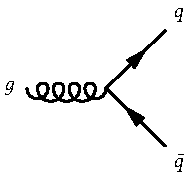
\includegraphics[width=0.7\textwidth]{gluon_quark_vertex}
%		\caption{\label{fig:gluon_quark_vertex}}
	\end{subfigure}%
	\begin{subfigure}[b]{0.30\linewidth}
		\centering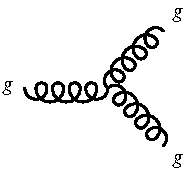
\includegraphics[width=0.7\textwidth]{gluon_vertex}
%		\caption{\label{fig:gluon_vertex}}
	\end{subfigure}	
	\begin{subfigure}[b]{0.30\linewidth}
		\centering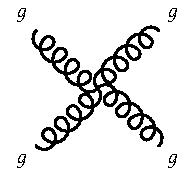
\includegraphics[width=0.7\textwidth]{gluon_quartic_vertex}
%		\caption{\label{fig:gluon_quartic_vertix}}
	\end{subfigure}
	\caption{Possible vertices in \gls{qcd}.}
	\label{fig:qcd_vertices}
\end{figure}

\subsubsection{Electroweak interaction}
\label{sec:ewk_interaction}

During the 1960s, Glashow, Weinberg and Salam~\cite{GLASHOW1961579,PhysRevLett.19.1264,Salam1959} developed a unified theory of the electromagnetic and weak interactions, based on the $SU(2)_\mathrm{L}\otimes U(1)_Y$ symmetry group. Known already experimentally from the Wu experiment~\cite{PhysRev.105.1413} in 1956, weak interaction violates parity, \ie the symmetry transformations have to act differently on the left-handed and right-handed fermion fields. The left- and right-handed components of a fermion field can be projected out using
\begin{equation}
	\psi_\mathrm{L} = \frac{1-\gamma^5}{2}\psi , \ \ \qquad 	\psi_\mathrm{R} = \frac{1+\gamma^5}{2}\psi,
\end{equation}
with $\gamma^5 = i\gamma^0\gamma^1\gamma^2\gamma^3$. As the weak interaction only acts on left-handed fermions, they can be ordered as $SU(2)$ doublets
\begin{equation}
	\begin{pmatrix}
		\nu_e \\
		e
	\end{pmatrix}_\mathrm{L},
	\quad
	\begin{pmatrix}
		u \\
		d
	\end{pmatrix}_\mathrm{L},
	\qquad
	\begin{pmatrix}
		\nu_\mu \\
		\mu
	\end{pmatrix}_\mathrm{L},
	\quad
	\begin{pmatrix}
		c \\
		s
	\end{pmatrix}_\mathrm{L},
	\qquad
	\begin{pmatrix}
		\nu_\tau \\
		\tau
	\end{pmatrix}_\mathrm{L},
	\quad
	\begin{pmatrix}
		t \\
		b
	\end{pmatrix}_\mathrm{L}.
\end{equation} 
The quantum number associated with $SU(2)$ symmetry transformations is called weak isospin $I$ with the third component denoted as $I_3$. Fermion doublets have $I=1/2$, with the upper component having $I_3 = 1/2$ and the lower component $I_3=-1/2$. Right-handed fermion fields have $I=0$, \ie are singlet states in weak isospin space
\begin{equation}
	e_\mathrm{R},\,  u_\mathrm{R},\,  d_\mathrm{R}, \qquad \mu_\mathrm{R},\,  c_\mathrm{R},\,  s_\mathrm{R}, \qquad \tau_\mathrm{R},\,  t_\mathrm{R},\,  b_\mathrm{R}, 
\end{equation}
and thus do not couple to the weak interaction. In the electroweak theory, neutrinos are assumed to be strictly massless, therefore no right-handed neutrino singlets exist. 

The fermion doublets can be written in a free Lagrangian similar to \cref{eq:free_lagrangian,eq:dirac_lagrangian},
\begin{equation}
	\Lagr = \bar{\psi}_\mathrm{L}i\gamma^\mu\uppartial_\mu\psi_\mathrm{L},
\end{equation}
with one crucial difference---the omission of the fermion masses. As $\bar{\psi}\psi = \bar{\psi}_\mathrm{L}\psi_\mathrm{R} + \bar{\psi}_\mathrm{R}\psi_\mathrm{L}$, mass terms would mix left- and right-handed terms and break gauge invariance. \Cref{sec:ssb} will illustrate how fermion masses will instead be generated in the electroweak theory. For left-handed fermion fields, local $SU(2)_\mathrm{L}$ transformations can be written as
\begin{equation}
	\psi_\mathrm{L} \rightarrow \mathrm{exp}\left(ig_2\alpha^a\frac{\sigma^a}{2}\right)\psi_\mathrm{L},
\end{equation}  
where $g_2$ is the coupling constant, $\alpha^a$ (with $a=1,2,3$) are real parameters and the Pauli matrices $\sigma^a$ are the generators of $SU(2)_\mathrm{L}$. By introducing the covariant derivative $\codiff_\mu = \uppartial_\mu + ig_2\frac{\sigma^a}{2}W^a_\mu$ and including the usual kinetic term for the gauge fields, the Lagrangian becomes invariant under $\mathrm{SU}(2)_\mathrm{L}$ transformations and reads
\begin{equation}
	\Lagr = \bar{\psi}_\mathrm{L}i\gamma^\mu\codiff_\mu\psi_\mathrm{L} - \frac{1}{4}W^a_{\mu\nu}W^{\mu\nu,a},
\end{equation}
with the gauge field strength tensors $W^a_{\mu\nu} = \uppartial_\mu W^a_\nu - \uppartial_\nu W^a_\mu + g_2 \epsilon^{abc}W^b_\mu W^c_\nu$, where $\epsilon^{abc}$ are the structure constants. As previously in the case of \gls{qcd}, the non-Abelian structure of the symmetry group causes self-interactions of the gauge fields.

In order to include electromagnetic interactions, the weak isospin group is extended with the $U(1)_Y$ group, corresponding to the multiplication of a phase factor $e^{i\alpha\frac{Y}{2}}$ to each of the preceding doublets and singlets. Here, $Y$ is the weak hypercharge as given by the Gell-Mann--Nishijima relation~\cite{Gell-Mann1956,10.1143/PTP.13.285,10.1143/PTP.10.581},
\begin{equation}
	Q = I_3 + \frac{Y}{2},
	\label{eq:gell-mann-nishijima}
\end{equation}
with $Q$ the electric charge.
As will be discussed in \cref{sec:ssb}, the spontaneous breaking of the \mbox{$SU(2)_\mathrm{L}\otimes U(1)_Y$} gauge symmetry will recover the electromagnetic gauge group $U(1)_\mathrm{em}$~\cite{Peskin:1995ev}.

By modifying the covariant derivative to include a $U(1)_Y$ gauge field and ensuring that $U(1)_Y$ acts the same on left-handed and right-handed fermions with coupling constant $g_1$, it can be written as $\codiff_\mu = \uppartial_\mu + ig_2\frac{\sigma^a}{2}W^a_\mu + ig_1\frac{Y}{2}B_\mu$ for left-handed fermions and $\codiff_\mu = \uppartial_\mu + ig_1\frac{Y}{2}B_\mu$ for right-handed fermions. The full electroweak Lagrangian then is
\begin{equation}
\begin{split}
	\Lagr_\mathrm{electroweak} = & \sum_j{\bar{\psi}_\mathrm{L}^j i \gamma^\mu \left(\uppartial_\mu -ig_2\frac{\sigma^a}{2} W^a_\mu + ig_1 \frac{Y}{2} B_\mu \right) \psi^j_\mathrm{L}} \\
	& + \sum_j{\bar{\psi}_\mathrm{R}^j i \gamma^\mu \left(\uppartial_\mu + ig_1 \frac{Y}{2} B_\mu \right) \psi^j_\mathrm{R}}, 
\end{split}
\end{equation}
where $B_{\mu\nu} = \uppartial_\mu B_\nu - \uppartial_\nu B_\mu$, and the two sums run over the left- and right-handed fermions, respectively.

\subsubsection{Spontaneous symmetry breaking}
\label{sec:ssb}

In the electroweak theory a total of three vector fields $W^a_\mu$ and one vector field $B_\mu$ are associated with the gauge groups $SU(2)_\mathrm{L}$ and $U(1)_Y$, respectively. As has been shown explicitly through the example of \gls{qed} in \cref{sec:gauge_principle}, the gauge fields need to be massless for the resulting Lagrangian to be gauge invariant under the respective symmetry group. In addition, the electroweak symmetry group does not allow for fermion masses. Both gauge bosons of the weak interaction and the fermions are, however, manifestly massive, and therefore the electroweak symmetry has to be broken in the \gls{sm}.

The spontaneous symmetry breaking of the $SU(2)_\mathrm{L}\otimes U(1)_Y$ gauge group is achieved through the Brout--Englert--Higgs   mechanism~\cite{PhysRevLett.13.321,PhysRevLett.13.508,PhysRev.145.1156}. In the SM, an isospin doublet of complex scalar fields, called Higgs doublet, is introduced
\begin{equation}
	\Phi(x) = \begin{pmatrix}
		\phi^+(x) \\
		\phi^0(x)
	\end{pmatrix}.
\end{equation}
The Higgs doublet has hypercharge $Y=1$, and thus, according to the Gell-Mann--Nishijima relation, $\phi^+$ has electric charge +1 while $\phi^0$ is electrically neutral. With the covariant derivative introduced in \cref{sec:ewk_interaction}, the Higgs doublet gets corresponding terms in the SM Lagrangian, 
\begin{equation}
	\Lagr_h = (\codiff_\mu\Phi)^\dagger(\codiff^\mu\Phi) - V(\Phi),
	\label{eq:higgs_lagrangian}
\end{equation}
where $V(\Phi)$ is a gauge invariant potential of the form
\begin{equation}
	V(\Phi) = -\mu^2\Phi^\dagger\Phi + \frac{\lambda}{4}(\Phi^\dagger\Phi)^2.
	\label{eq:higgs_potential}
\end{equation}
For positive and real parameters $\mu^2$ and $\lambda$, this potential has the form of a \textit{Mexican hat} and an infinite number of minima for field configurations with $\Phi^\dagger\Phi=2\mu^2/\lambda$. In the vacuum, \ie in the ground state of the theory with minimal potential energy of the field, one of these minima is chosen such that the Higgs  receives a \gls{vev},
\begin{equation}
	\braket{\Phi} = \frac{1}{\sqrt{2}}\begin{pmatrix}
		0 \\
		v
	\end{pmatrix} \qquad \textrm{with} \quad v = \frac{2\mu}{\sqrt{\lambda}} \approx \SI{246}{\GeV}.
	\label{eq:higgs_vev}
\end{equation}
\Cref{eq:higgs_vev} is neither invariant under a $SU(2)_\mathrm{L}$ transformation of the form $U = \mathrm{exp}(i\alpha^a\frac{\sigma^a}{2})$, nor under a $U(1)_Y$ phase factor of the form $\mathrm{exp}(i\alpha\frac{Y}{2})$. Thus, the Lagrangian has a symmetry that the vacuum state does not share, thereby spontaneously breaking the $SU(2)_\mathrm{L}\otimes U(1)_Y$ symmetry. As the \gls{vev} of $\phi^+$ vanishes and $\phi^0$ is invariant under $U(1)_\mathrm{em}$, the $SU(2)_\mathrm{L}\otimes U(1)_Y$ symmetry group is broken down to $U(1)_\mathrm{em}$~\cite{Brock:1354959}.

The Higgs doublet can be expressed as excitations around the ground state
\begin{equation}
	\Phi(x) = \frac{1}{\sqrt{2}} \begin{pmatrix}
		\phi_1(x)+i\phi_2(x) \\
		v + h(x) + i\chi(x)
	\end{pmatrix},
	\label{eq:higgs_expansion}
\end{equation}
where $h$, $\chi$, $\phi_1$ and $\phi_2$ are real-valued scalar fields with vanishing \glspl{vev}. Inserting 
\cref{eq:higgs_expansion} back into the potential $V(\Phi)$ in \cref{eq:higgs_potential} yields
\begin{equation}
	V = \mu^2h^2 + \frac{\mu^2}{v} h (h^2 + \chi^2 + \phi_1^2+\phi_2^2)+ \frac{\mu^2}{4v^2}(h^2 + \chi^2 + \phi_1^2 + \phi_2^2),
	\label{eq:higgs_potential_excitation}
\end{equation}
where only \textit{h} gets a mass term, thus corresponding to an electrically neutral scalar particle with mass $m_h = \sqrt{2}\mu$.
The other scalar fields remain massless, which is in accordance with the Nambu-Goldstone theorem~\cite{Nambu:1960tm,Goldstone:1961eq}, stating that every spontaneously broken continuous symmetry generates a massless Goldstone boson. These bosons are unphysical and can be gauged away through a $SU(2)_\mathrm{L}$ transformation, such that the expansion around the vacuum from \cref{eq:higgs_expansion}, involves only the physical scalar $h$ in the so-called \textit{unitary gauge}~\cite{Brock:1354959}.
\begin{figure}
	\centering
	\begin{subfigure}[b]{0.30\linewidth}
		\centering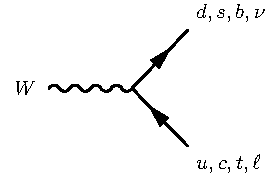
\includegraphics[width=0.8\textwidth]{w_fermion_vertex}
	\end{subfigure}
	\begin{subfigure}[b]{0.30\linewidth}
		\centering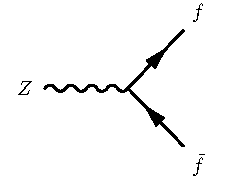
\includegraphics[width=0.8\textwidth]{z_fermion_vertex}
	\end{subfigure}
	\begin{subfigure}[b]{0.30\linewidth}
		\centering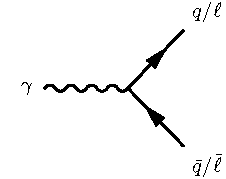
\includegraphics[width=0.8\textwidth]{gamma_fermion_vertex}
	\end{subfigure}
	\par\medskip
	\begin{subfigure}[b]{0.30\linewidth}
		\centering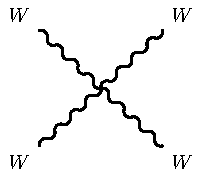
\includegraphics[width=0.7\textwidth]{w_boson_quartic_vertex}
	\end{subfigure}
	\begin{subfigure}[b]{0.30\linewidth}
		\centering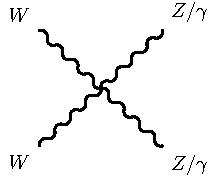
\includegraphics[width=0.7\textwidth]{wz_boson_quartic_vertex}
	\end{subfigure}	
	\begin{subfigure}[b]{0.30\linewidth}
		\centering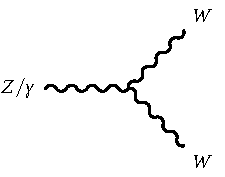
\includegraphics[width=0.8\textwidth]{w_boson_cubic_vertex}
	\end{subfigure}
	\caption{Possible vertices in the electroweak interaction.}
	\label{fig:ewk_vertices}
\end{figure}


Inserting \cref{eq:higgs_expansion} and the potential $V$ from \cref{eq:higgs_potential_excitation} back into the Lagrangian $\Lagr_h$ in \cref{eq:higgs_lagrangian} leads to mass terms for the gauge fields through their couplings to the \textit{h} field. The \textit{physical} fields corresponding to the physically observable $W^\pm$, $Z$ and $\gamma$ bosons in the electroweak theory are then given by the linear combinations
\begin{align*}
	W^\pm_\mu 	& = \frac{1}{\sqrt{2}}(W^1_\mu\mp i W^2_\mu) 				& \textrm{with} \quad m_W  & = \frac{g_2}{2}v, \\
	Z_\mu 		& = \cos\theta_W W_\mu^3 - \sin\theta_W B_\mu 	& \textrm{with} \quad m_Z  & = \frac{1}{2}\sqrt{g_1^2+g_2^2}v, \\
	A_\mu 		& = \sin\theta_W W_\mu^3 + \cos\theta_W B_\mu 	& \textrm{with} \quad m_A  & = 0,
\end{align*}
where $\theta_W$ is the weak mixing angle. It is related to the masses of the $W$ and $Z$ bosons and the electroweak coupling constants by
\begin{equation}
	\cos{\theta_W} = \frac{g_2}{\sqrt{g_1^2 + g_2^2}} = \frac{m_W}{m_Z}.
\end{equation} 

%The Higgs potential can then be written as
%\begin{equation}
%	V = \mu^2h^2 + \frac{\mu^2}{v} h (h^2 + \chi^2 + \phi_1^2+\phi_2^2)+ \frac{\mu^2}{4v^2}(h^2 + \chi^2 + \phi_1^2 + \phi_2^2),
%\end{equation}
%where only $h$ gets a mass term, thus describing an electrically neutral scalar particle with mass $m_h = \sqrt{2}\mu$. The remaining scalar fields remain massless, in accordance with the Nambu-Goldstone theorem~\cite{Nambu:1960tm,Goldstone:1961eq}, stating that every spontaneously broken continuous symmetry generates a massless Goldstone boson. These bosons are unphysical and can be gauged away through a $SU(2)_\mathrm{L}$ transformation, such that the expansion around the vacuum from \cref{eq:higgs_expansion} involves only the physical scalar $H(x)$,
%\begin{equation}
%	\Phi(x) = \frac{1}{\sqrt{2}} \begin{pmatrix}
%		0 \\
%		v + h(x)
%	\end{pmatrix}.	
%\end{equation}
%The gauge transformation bringing \cref{eq:higgs_expansion} into the above form is called the \textit{unitary gauge}~\cite{Brock:1354959}. In this gauge, the Higgs potential from \cref{eq:higgs_potential} has the form
%\begin{equation}
%	V = \frac{m_h^2}{2} h^2 + \frac{m_h^2}{2v} h^3 + \frac{m_h^2}{8v^2} h^4,
%\end{equation}
%containing cubic and quartic self-interactions of the Higgs field proportional to $m^2_h$. Inserting the excitation around the vacuum state in the kinetic term of $\Lagr_\mathrm{h}$ yields mass terms for the vector bosons,
%\begin{equation}
%	\Lagr_{h} \propto \frac{v^2}{8}g^2_2\left(W_\mu^1W^{1,\mu} + W_\mu^2W^{2,\mu}\right) + \frac{v^2}{8} \begin{pmatrix}
%		W^3_\mu & B_\mu
%	\end{pmatrix}
%	\begin{pmatrix}
%		g_2^2 & g_1g_2   \\
%		g_1g_2 & g_1^2
%	\end{pmatrix}
%	\begin{pmatrix}
%		W^{3,\mu} \\
%		B^\mu
%	\end{pmatrix}.
%\end{equation}
%Instead of expressing the Lagrangian in terms of the fields $W^a_\mu$ and $B_\mu$ that make the original gauge invariance manifest, it can also be written in terms of the \textit{physical} fields that correspond to the physical $W^\pm$, $Z$ and $\gamma$ bosons in the electroweak theory,
%\begin{align*}
%	W^\pm_\mu 	& = \frac{1}{\sqrt{2}}(W^1_\mu\mp i W^2_\mu) 				& \textrm{with} \quad m_W  & = \frac{g_2}{2}v, \\
%	Z_\mu 		& = \frac{1}{\sqrt{g_1^2+g_2^2}}(g_2W^3_\mu - g_1 B_\mu) 	& \textrm{with} \quad m_Z  & = \frac{\sqrt{g_1^2+g_2^2}}{2}v, \\
%	A_\mu 		& = \frac{1}{\sqrt{g_1^2+g_2^2}}(g_1W^3_\mu + g_2 B_\mu) 	& \textrm{with} \quad m_A  & = 0.
%\end{align*}
%It is worth noting, that the massless photon field $A_\mu$ associated with the electromagnetic $U(1)_\mathrm{em}$ gauge symmetry is automatically recovered. All possible vertices between fermions and the physical electroweak gauge bosons are shown in \cref{fig:ewk_vertices}. The change of basis from $(W^3_\mu, B_\mu)$ to $(Z_\mu,A_\mu)$~\cite{Peskin:1995ev} can also be written as a basis rotation with the weak mixing angle $\theta_W$, \improvement{Write somewhere SU2xU1 to U1 breakdown}
%\begin{equation}
%	\begin{pmatrix}
%		Z_\mu \\
%		A_\mu
%	\end{pmatrix} =
%	\begin{pmatrix}
%		\cos{\theta_W} & \sin{\theta_W} \\
%		- \sin{\theta_W} & \cos{\theta_W}
%	\end{pmatrix}
%	\begin{pmatrix}
%		W^3_\mu \\
%		B_\mu
%	\end{pmatrix} \qquad \textrm{with } \cos{\theta_W} = \frac{g_2}{\sqrt{g_1^2 + g_2^2}} = \frac{m_W}{m_Z}.
%\end{equation}

\begin{figure}
	\centering
	\begin{subfigure}[b]{0.30\linewidth}
		\centering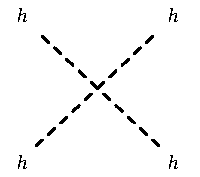
\includegraphics[width=0.75\textwidth]{h_boson_quartic_vertex}
	\end{subfigure}%
	\begin{subfigure}[b]{0.30\linewidth}
		\centering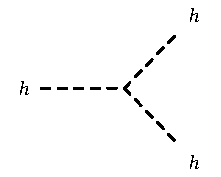
\includegraphics[width=0.85\textwidth]{h_boson_cubic_vertex}
	\end{subfigure}%
	\begin{subfigure}[b]{0.30\linewidth}
		\centering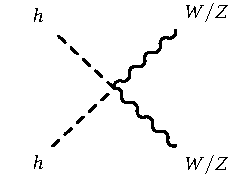
\includegraphics[width=0.9\textwidth]{h_boson_digauge_vertex}
	\end{subfigure}
	\par\medskip
	\begin{subfigure}[b]{0.30\linewidth}
		\centering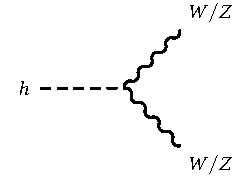
\includegraphics[width=0.9\textwidth]{h_boson_gauge_vertex}
	\end{subfigure}%
	\begin{subfigure}[b]{0.30\linewidth}
		\centering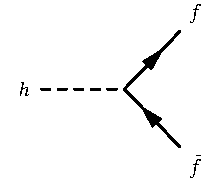
\includegraphics[width=0.85\textwidth]{h_boson_fermion_vertex}
	\end{subfigure}	
	\caption{Possible vertices involving the Higgs boson.}
	\label{fig:higgs_vertices}
\end{figure}

In the \gls{sm} the $W^\pm$ and $Z$ bosons hence acquire masses through spontaneous breaking of the electroweak gauge symmetry $SU(2)_\mathrm{L}\otimes U(1)_Y$ through the Higgs mechanism. The massless photon field $A_\mu$ associated with the electromagnetic $U(1)_\mathrm{em}$ gauge symmetry is automatically recovered. All possible vertices between fermions and the physical gauge bosons described by the electroweak theory are shown in \cref{fig:ewk_vertices}. 

Furthermore, the masses of fermion fields are related to gauge-invariant Yukawa interactions with the Higgs field. For one fermion generation, the respective Yukawa terms in the Lagrangian are
\begin{equation}
	\Lagr_\mathrm{Yukawa,gen} = - \lambda_\ell \bar{L}_\mathrm{L}\Phi\ell_\mathrm{R} - \lambda_d \bar{Q}_\mathrm{L}\Phi d_\mathrm{R} - \lambda_u \bar{Q}_\mathrm{L} \Phi^\dagger u_\mathrm{R} + \mathrm{h.c.},
\end{equation}
where $\lambda_f$ with $f = \ell,d,u$ are the dimensionless Yukawa couplings and $L_\mathrm{L} = (\nu_\mathrm{L},\ell_\mathrm{L})^T$ and $Q_\mathrm{L} = (u_\mathrm{L},d_\mathrm{L})^T$ are the left-handed lepton and quark doublets, respectively. The non-vanishing \gls{vev} of the Higgs field then gives rise to fermion mass terms of the form 
\begin{equation}
 m_f = \lambda_f \frac{v}{\sqrt{2}},
\end{equation}
yielding fermion couplings to the Higgs field proportional to the fermion masses $m_f$. All \gls{sm} interaction vertices involving the Higgs boson are shown in \cref{fig:higgs_vertices}.
% The \gls{vev} of the Higgs field then gives rise to fermion mass terms in the Lagrangian, which, in the unitary gauge, yields for a single fermion generation
%\begin{equation}
% 	\Lagr_\mathrm{Yukawa, gen} = - \sum_{f=\ell,d,u}{\left(m_f\bar{\psi}_f\psi_f + \frac{m_f}{v}h\bar{\psi}_f\psi_f\right)} \qquad \textrm{with} \quad m_f = \frac{1}{\sqrt{2}}\lambda_f v.
%\end{equation}

When introducing all three fermion generations, additional Yukawa terms mixing fermions of different generations appear in the Lagrangian~\cite{Brock:1354959}. The terms involving quark fields can be parametrised using the \gls{ckm} matrix~\cite{PhysRevLett.10.531,CKM:1973fv}, quantifying the transition probability between quark generations. Since no right-handed neutrinos exist in the SM, no generation mixing in the lepton sector occurs and hence no neutrino mass terms are allowed in the \gls{sm}. Neutrino oscillations have, however, been observed experimentally, thus at least two massive neutrino generations need to exist. Their mixing can be described\footnote{Technically, this is already an extension of the \gls{sm}.} with the \gls{pmns} matrix~\cite{PMNS:1962mu}, allowing neutrinos to acquire mass \eg through the see-saw mechanism~\cite{Brdar:2019iem}.
 
\subsection{Renormalisation and divergencies}
\label{ch:renormalisation}

At lowest order in the perturbative expansion, the momenta of the internal lines in the Feynman diagrams are fixed by the external particles. For higher orders where the diagrams involve loops, the momenta of the internal lines need to be integrated over as they are not fixed by energy-momentum conservation. Some examples of loop corrections to propagators and vertices are shown in \cref{fig:loop_corrections}. As each vertex in the Feynman diagrams is associated with a coupling constant that is usually much smaller than 1 (apart from the non-perturbative regime of \gls{qcd}), higher orders in the perturbative expansion contribute less and less to the total amplitude of the full expansion.

\begin{figure}
	\centering
	\begin{subfigure}[b]{0.33\linewidth}
		\centering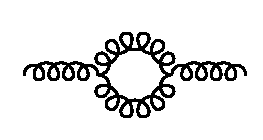
\includegraphics[width=0.85\textwidth]{gluon_loop}
		\caption{\label{fig:gluon_loop}}
	\end{subfigure}%
	\begin{subfigure}[b]{0.33\linewidth}
		\centering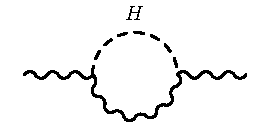
\includegraphics[width=0.85\textwidth]{wz_propagator}
		\caption{\label{fig:wz_propagator}}
	\end{subfigure}	
	\begin{subfigure}[b]{0.33\linewidth}
		\centering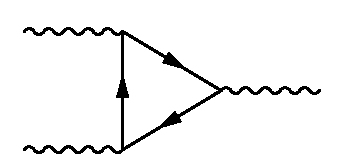
\includegraphics[width=0.85\textwidth]{cubic_vertex}
		\caption{\label{fig:cubic_vertex}}
	\end{subfigure}
	\caption{Examples of loop corrections to (a) the gluon propagator, (b) the $W$ or $Z$ propagator and (c) the cubic gauge boson vertex.}\label{fig:loop_corrections}
\end{figure}

The momentum integrals in loop corrections, however, lead to \textit{ultraviolet divergencies} for large momenta. In order to eliminate the divergencies, the integrals have to be \textit{regularised}, \eg by applying a cut-off scale $\Lambda$, or calculating the integrals in a number $D = 4-\epsilon$ of dimensions where they converge. The potential divergencies are then absorbed in parameters of the Lagrangian, such as coupling constants and masses, after which the regulator is removed again (\eg by setting $\epsilon\rightarrow 0$) and a \textit{renormalisation} procedure is applied, replacing the bare parameter values with the physical, measured values~\cite{Brock:1354959}. Renormalisation effectively absorbs the effects of quantum fluctuations, acting on much smaller scales than the scale of the given problem, into the parameters of the theory.
 As Veltmann and t'Hooft~\cite{THOOFT1972189,THOOFT1971173} have shown, all Yang-Mills theories with massive gauge fields are renormalisable, rendering the \gls{sm} as a whole a renormalisable theory.  

\section{Supersymmetry}

Originally developed in the late 1960s and early 1970s as an attempt to combine the Poincaré group with internal symmetries into a single symmetry group~\cite{kane2000the}, \glsfirst{susy} is a class of theories transforming fermionic states into bosonic ones, and vice-versa. Since its theoretical discovery, driven purely by theoretical developments rather than by pressure of existing data~\cite{kane2000the}, \gls{susy} was found to have far-reaching phenomenological consequences that could solve some of the shortcomings of the \gls{sm}. 

This section starts with an overview of the shortcomings of the \gls{sm} and illustrates how they could be solved by supersymmetric theories. This is followed by an introduction to the mathematical description and phenomenological consequences of \gls{susy}. While the following sections are intended to highlight the most important concepts and relations, a much more complete and detailed introduction to \gls{susy} can be found, \eg, in \references\cite{Martin:1997ns,Bustamante:2009us}.

%Among the properties a quantum field theory might possess to make it more mathematically tractable, one specific higher symmetry reveals particularly far-reaching implications; a symmetry relating fermions and bosons, known as \gls{susy}. In the following, the basic concepts of \gls{susy}, a class of theories that could solve some of the shortcomings of the \gls{sm}. 

%First, some of the shortcomings of the \gls{sm} are highlighted, and possible solutions through supersymmetric theories are illustrated.  highlighting some of the open questions of the SM. This is followed by an introduction to the mathematical description and phenomenological consequences of supersymmetric theories. The following sections are intended to highlight the most important concepts and relations, a much more complete and detailed introduction to \gls{susy} can be found in \references\cite{Martin:1997ns,Bustamante:2009us}.

\subsection{Shortcomings of the Standard Model}\label{sec:shortcomings_sm}

Although the \gls{sm} is a remarkably successful theory that is able to predict and describe the interactions between elementary particles with unprecedented precision, there are still phenomena in nature that cannot be suitable understood within the theoretical framework of the \gls{sm}. 

Those limitations and open questions are the reason for numerous searches looking for new physics beyond the \gls{sm}, such as the one presented in this thesis. Some of these open questions are described in the following. 

\subsubsection{Dark Matter}

The existence of \glsfirst{dm}, \ie non-luminous and non-absorbing matter is nowadays well established~\cite{pdg2020}. Some of the earliest hints for the existence of \gls{dm} came from the observation that the rotation curves of luminous objects are not consistent with the expected velocities based on the gravitational attraction of the visible objects around them. Zwicky already postulated in 1933 the existence of \gls{dm}~\cite{Zwicky:437297} based on rotation curves of galaxies in the Coma cluster. In 1970, Rubin measured rotation curves of spiral galaxies~\cite{Rubin:1970zza}, revealing again a significant disagreement with the theoretically expected curves given the visible matter in the galaxies. Based on Newtonian dynamics, the circular velocity of stars outside the bulge of galaxies is expected to fall off with increasing radius as $v(r) \propto 1/\sqrt{r}$~\cite{Bertone:2004pz}. Rubin's observations, however, revealed that the velocities of stars outside the bulge stay approximately constant, strongly suggesting the existence of a non-luminous (or \textit{dark}) matter halo around the galaxies. Surveys of galaxy clusters and observations of gravitational lensing effects, \eg, in the bullet cluster~\cite{Clowe:2006eq} or the Abell 1689 cluster~\cite{Taylor:1998uk}, have since then further consolidated the existence of large accumulations of non-luminous matter in the universe.

The anisotropies in the \gls{cmb}, studied by the COBE~\cite{Bennett:1996ce,COBE}, WMAP~\cite{WMAP2,WMAP1} and Planck missions~\cite{Planck} are well described by the \gls{lcdm} model~\cite{Liddle:1976476}, which includes a density for cold dark matter. Planck's latest results~\cite{Aghanim:2018eyx} for the cold \gls{dm} relic density $\Omega_c h^2$ and baryonic density $\Omega_b h^2$ of
\begin{align}
\begin{split}
	\Omega_c h^2 &= 0.1200\pm0.0012, \\
	\Omega_b h^2 &= 0.02237\pm0.00015,
\end{split}
\end{align}
suggest that ordinary baryonic matter only makes up $\sim 4.9\%$ of the universe's matter content, while \gls{dm} accounts for $\sim 26.1\%$. The remaining $\sim 69\%$ are taken up by \textit{dark energy}, the nature of which is yet another open question.

Candidates for cold \gls{dm} need to satisfy certain conditions: they have to be stable on cosmological timescales (otherwise they would have decayed by now), they have to couple only very weakly to the electromagnetic interaction (if at all, otherwise they would be \textit{luminous} matter) and they need to have the right relic density. Analyses of structure formations in the Universe have furthermore shown that most \gls{dm} should have been \textit{cold}, \ie non-relativistic, at the beginning of galaxy formation~\cite{Bertone:2004pz}. Candidates for \gls{dm} particles are \eg sterile neutrinos, axions, primordial black holes, or \glspl{wimp}.

In the SM, the only \gls{dm} candidate particle is the neutrino. Given the upper limits on the neutrino masses, an upper bound on their relic density can be computed, revealing that neutrinos are not abundant enough to be a dominant component of \gls{dm}~\cite{Bertone:2004pz}. Furthermore, due to their low masses, neutrinos would still have been relativistic particles at the beginning of galaxy formation, preventing the \textit{bottom-up}\footnote{The \textit{bottom-up} structure formation begins with small objects that subsequently merge into ever larger structures and corresponds to the structure formation process favoured in a universe dominated by cold \gls{dm}.} structure formation, favoured by a cold \gls{dm} dominated universe.

 Many \gls{bsm} theories naturally predict new \glspl{wimp} with masses in the GeV to TeV range. In many \gls{susy} models with exact R-parity conservation (a quantity introduced in \cref{sec:rparity}), the lightest supersymmetric particle is neutral and stable and could be a good candidate for \gls{dm}.

\subsubsection{Unification of forces}


Although the \gls{sm} provides a good description of nature up to the energy scale probed with today's accelerators, some of its peculiar aspects hint to a more fundamental theory. A prominent example is the question why the electric charges of the electrons and the charges of the quarks in the protons and neutrons in the nuclei exactly cancel, making for electrically neutral atoms~\cite{Brock:1354959}. Or in other words: why are the charges of all observed particles simple multiples of the fundamental charge? And why are they quantised in the first place?

An explanation to many of these peculiarities comes naturally when describing the \gls{sm} as a unified theory with a single non-Abelian gauge group, \eg $SU(5)$~\cite{PhysRevLett.32.438}. The larger symmetry group with a single coupling constant is then thought to be spontaneously broken at very high energy, such that the known \gls{sm} interactions are recovered at the lower energies probed in today's experiments. In such a \gls{gut}, the particles in the \gls{sm} are arranged in anomaly-free\footnote{In the sense that loop corrections do not break symmetries that the Lagrangian has.}, irreducible representations of the gauge group, thereby, for example, naturally ensuring the fractional charges of quarks~\cite{Peskin:1995ev}.

\begin{figure}
\floatbox[{\capbeside\thisfloatsetup{capbesideposition={right,center},capbesidewidth=0.4\textwidth}}]{figure}[\FBwidth]
{\caption{Evolution of the inverse coupling constants in the \gls{sm} (dashed lines) and the \gls{mssm} (solid lines) in function of the energy scale $Q$. Here, the masses of the supersymmetric particles are treated as common threshold and varied between $\SI{750}{\GeV}$ (blue lines) and $\SI{2.5}{\TeV}$ (red lines). Figure taken from \reference\cite{Martin:1997ns}.}\label{fig:unification_forces}}
{\includegraphics[width=0.5\textwidth]{unification}}
\end{figure}

In the \gls{sm}, the coupling constants run towards each other with increasing energy scale, but never exactly meet. In the \glsfirst{mssm}, introduced in \cref{sec:mssm_intro}, the running couplings meet within their current uncertainties if the supersymmetric particles are at the $\SI{}{\TeV}$ scale, hinting that a supersymmetric \gls{gut} could be a good candidate for describing physics at the unification scale. \Cref{fig:unification_forces} shows that the running coupling constants in the \gls{mssm} are modified such that they meet at $\SI{e16}{\GeV}$.

\subsubsection{The Hierarchy Problem}

As the \gls{sm} is a renormalisable gauge theory, finite results are obtained for all higher-order loop corrections, making the \gls{sm} a theory that is, in principle, well-defined up to infinite energies. In renormalisation terms, this means that the cut-off scale $\Lambda$ is theoretically allowed to go to arbitrarily high values. It is clear though, that the \gls{sm} cannot be a complete theory of nature and that, at some unknown high-energy scale $\Lambda$, \textit{new physics} has to appear. At the very least, a new theoretical framework becomes necessary at the Planck scale $M_P \approx \SI{e19}{\GeV}$~\cite{Bustamante:2009us}, where quantum gravitational effects can no longer be ignored.

The mass parameters of fermions and massive vector bosons are protected from large quantum corrections by chiral symmetry and gauge symmetry, respectively~\cite{Aitchison:2007fn}. The mass parameter of the scalar Higgs field, on the other hand, receives loop corrections proportional at least to the scale at which new physics sets in. The Yukawa coupling of the Higgs field to a fermion $f$ with mass $m_f$, depicted in \cref{fig:fermion_loop}, yields a one-loop correction term to the Higgs square mass~\cite{Bustamante:2009us} given by
\begin{align}
	\upDelta m_h^2 = -\frac{\lambda_f^2}{8\uppi^2} \Lambda^2 + \dots\, .
	\label{eq:fermion_correction}
\end{align}
The Higgs mass thus quadratically diverges with the scale $\Lambda$. If the \gls{sm} is to be valid up to the Planck scale, then $\Lambda = M_P$, and the correction to the Higgs squared mass becomes more than $10^{30}$ times larger than the expected value in the order of $(\SI{e2}{\GeV})^2$~\cite{Martin:1997ns}.
Similar quantum corrections arise from the Higgs quartic coupling to a heavy scalar boson $S$ with mass $m_S$, shown in \cref{fig:scal_loop}, yielding a one-loop correction~\cite{Bustamante:2009us} given by 
\begin{align}
	\upDelta m_h^2 = \frac{\lambda_S}{16\uppi^2}\Lambda^2 + \dots\, .
	\label{eq:scalar_correction}
\end{align}
In order to obtain the experimentally measured value of the Higgs mass, the quantum corrections to the bare Higgs parameter have to be tuned in such a way that they almost cancel, leading to a \textit{fine-tuning} problem that is considered to be unnatural.

Interestingly, the terms quadratically divergent in $\Lambda$ in \cref{eq:fermion_correction} and \cref{eq:scalar_correction} enter with opposite signs. If, for every fermionic loop, there are two bosonic loops with $\lambda_S = \lambda_f^2$, the quadratically diverging terms neatly cancel. As will be discussed, this is exactly the case in supersymmetric theories. Additional correction terms omitted above are at most logarithmic in $\Lambda$, and cancel if the scalar bosons and the fermion have the same masses (this is further discussed in \cref{sec:susy_breaking}).

\begin{figure}
	\centering
	\begin{subfigure}[b]{0.5\linewidth}
		\centering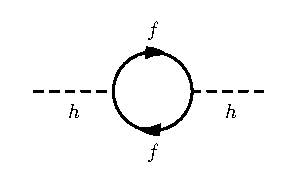
\includegraphics[width=0.75\textwidth]{fermion_loop}
		\caption{\label{fig:fermion_loop}}
	\end{subfigure}%
	\begin{subfigure}[b]{0.5\linewidth}
		\centering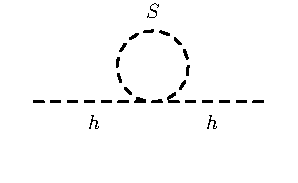
\includegraphics[width=0.75\textwidth]{scalar_loop}
		\caption{\label{fig:scal_loop}}
	\end{subfigure}	
	\caption{A massive fermion \subref{fig:fermion_loop} and a hypothetical massive scalar particle \subref{fig:scal_loop} coupling to the Higgs boson.}\label{fig:loop_corrections_higgs}
\end{figure}

%In SUSY, the Higgs mass is automatically protected from the large quantum corrections by the introduction of two complex scalar partners to each \gls{sm} fermion. The quantum corrections from a hypothetical heavy complex scalar particle $S$ with mass $m_S$ as in \cref{fig:scal_loop} yields a one-loop correction~\cite{Martin:1997ns} given by 
%\begin{align}
%	\upDelta m_h^2 = \frac{\lambda_S}{16\uppi^2}\left[\Lambda^2 - 2m_S^2\ln\left(\Lambda/m_S\right)+ \dots\right].
%	\label{eq:scalar_correction}
%\end{align}

%Interestingly, the corrections in \cref{eq:fermion_correction} and \cref{eq:scalar_correction} enter with opposite signs. Thus, if $\lambda_S = \vert\lambda_f\vert^2$, then the large quantum corrections neatly cancel and no excessive fine-tuning is needed. The requirement $\lambda_S = \vert\lambda_f\vert^2$ means that the fermions and their supersymmetric bosonic partners would have same masses. Such particles would have been discovered long ago in particle physics experiments, meaning that SUSY must be a broken symmetry (see \cref{sec:susy_breaking} for a discussion on \gls{susy} breaking) such that the supersymmetric particles acquire masses well above those of their \gls{sm} partners. 

\subsubsection{Anomalous magnetic moment of the muon}

One of the longest standing disagreements between experiment and theory in the \gls{sm} is the anomalous magnetic moment of the muon~\cite{pdg2020}. The magnetic moment of the muon $\vec{\mu}_\mu$ is related to its intrinsic spin $\vec{S}$ through the gyromagnetic ratio $g_\mu$ by
\begin{equation}
	\vec{\mu}_\mu = g_\mu \frac{q}{2m} \vec{S}.
\end{equation}
For a structureless spin-1/2 particle with mass $m$ and charge $q=\pm e$, the gyromagnetic ratio is \mbox{$g_\mu = 2$} \cite{Bennett:2006fi}. Loop corrections coupling the muon spin to virtual fields cause small deviations, parameterised by the anomalous magnetic moment
\begin{equation}
	a_\mu = \frac{1}{2}(g_\mu-2).
\end{equation}
The anomalous magnetic moment can be precisely predicted within the SM and experimentally measured with high accuracy. A comparison between experimental data and theoretical prediction thus directly tests the \gls{sm} at quantum loop level and may hint to effects from new physics in case of discrepancies~\cite{baer_tata_2006}.
In the SM, the most dominant contribution to $a_\mu$ comes from \gls{qed} corrections involving photon and fermion loops.
A representative diagram is shown in \cref{fig:qed_anomalous_moment}. Weak contributions involving the heavy $W^\pm$, $Z$ and Higgs particles are suppressed by their masses~\cite{Aoyama:2020ynm}.
Although the contributions from \gls{qcd} are relatively small, they give rise to the main theoretical uncertainties, since they cannot be calculated from first principles but rely either on data-driven calculations or lattice \gls{qcd} evaluations~\cite{Aoyama:2020ynm}.

The muon $g$--2 experiment at the Fermi National Accelerator Laboratory (FNAL)~\cite{Abi:2021gix} has recently measured the anomalous magnetic moment of the muon, updating the results from the E821 experiment at Brookhaven National Laboratory (BNL)~\cite{Bennett:2006fi}, obtained in 2004. The combined experimental average of both experiments finds a deviation from the \gls{sm} expectation\footnote{The \gls{sm} value of $a_\mu$ adopted in \reference\cite{Abi:2021gix} relies on the data-driven evaluation of the hadronic contributions using $e^+e^-$ collider data, recommended by the muon $g$--2 theory initiative~\cite{Aoyama:2020ynm}.} of
\begin{equation}
	\upDelta a_\mu = a^\mathrm{exp}_\mu - a^\mathrm{SM}_\mu = (251\pm59)\times 10^{-11},
%	\upDelta a_\mu = a^\mathrm{exp}_\mu - a^\mathrm{SM}_\mu = 261(63)(48)\times 10^{-11},
\end{equation}
which is quantified to have a significance of $4.2\sigma$~\cite{Abi:2021gix}. These results strongly hint at the existence of new physics beyond the \gls{sm}.

\begin{figure}
	\centering
	\begin{subfigure}[b]{0.33\linewidth}
		\centering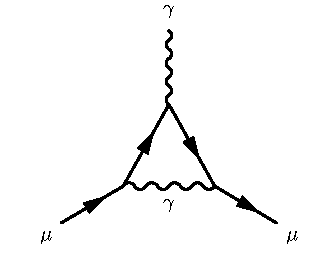
\includegraphics[width=1.0\textwidth]{qed_anomalous_moment}
		\caption{\label{fig:qed_anomalous_moment}}
	\end{subfigure}%
	\begin{subfigure}[b]{0.33\linewidth}
		\centering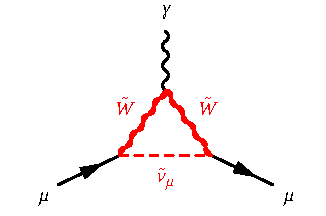
\includegraphics[width=1.0\textwidth]{susy_anomalous_moment_1}
		\caption{\label{fig:susy_anomalous_moment_1}}
	\end{subfigure}%
	\begin{subfigure}[b]{0.33\linewidth}
		\centering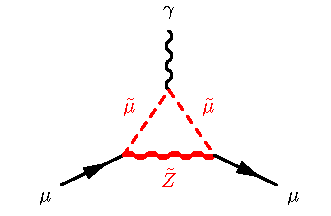
\includegraphics[width=1.0\textwidth]{susy_anomalous_moment_2}
		\caption{\label{fig:susy_anomalous_moment_2}}
	\end{subfigure}	
	\caption{Electromagnetic \subref{fig:qed_anomalous_moment} and supersymmetric \subref{fig:susy_anomalous_moment_1}, \subref{fig:susy_anomalous_moment_2} contributions to $a_\mu$. Supersymmetric particles are drawn in red. Adapted from~\reference\cite{baer_tata_2006}.}\label{fig:loop_corrections_anomalous_moment}
\end{figure}

In many supersymmetric models, the measured deviation in $a_\mu$ can easily be accommodated through additional Feynman diagrams involving the supersymmetric partners of the muon, the muon neutrino and the electroweak gauge bosons~\cite{Czarnecki:2001pv,Feng:2001tr}. Two lowest-order diagrams involving supersymmetric particles (introduced in \cref{sec:mssm_particle_content}) are shown in \cref{fig:susy_anomalous_moment_1,fig:susy_anomalous_moment_2}.


\subsection{Supersymmetric Algebra}\label{sec:susy_algebra}

The Coleman--Mandula no-go theorem~\cite{PhysRev.159.1251} dictates that the symmetry group generating a consistent spacetime \gls{qft} must be the direct product of the internal symmetry group with the Poincaré group, which in principle rules out the possibility for SUSY. The Coleman--Mandula proof, however, assumes the new symmetry to be generated by bosonic integer spin generators. The Haag--Lopuszanski--Sohnius extension~\cite{Haag:1974qh} showed that the only possible way of non-trivially combining internal and spacetime symmetry groups is to use a Lie superalgebra and fermionic spin-1/2 generators.

A generator of supersymmetric transformations is thus an anti-commuting spinor $Q$ that turns fermionic states $\ket{f}$ into bosonic states $\ket{b}$ and vice-versa,
\begin{equation}
	Q\ket{f} = \ket{b}, \qquad \qquad \qquad Q\ket{b}=\ket{f}.
\end{equation}
As spinors are complex objects, $Q^\dagger$ is also a symmetry operator. In order to obey the Haag--Lopuszanski--Sohnius loophole of the Coleman--Mandula theorem, both $Q$ and $Q^\dagger$ are necessarily fermionic and thus must carry half-integer spin, meaning that \gls{susy} must be a spacetime symmetry, \ie a Poincaré symmetry. To simultaneously allow for parity-violating interactions, the \gls{susy} generators have to satisfy the following algebra of commutation and anti-commutation relations~\cite{Bustamante:2009us},
\begin{equation}
\begin{split}
	\{ Q,Q^\dagger \} & \quad = \quad  2\sigma_\mu P^\mu,\\
	\{ Q,Q \} &  \quad = \quad \{ Q^\dagger,Q^\dagger \} = 0, \\
	\left[P^\mu,Q \right] &  \quad = \quad \left[ P^\mu,Q^\dagger \right] = 0, \\
	\{ M^{\mu\nu}, Q \} & \quad = \quad \sigma^{\mu\nu} Q,\\
	\{ M^{\mu\nu},Q^\dagger \} & \quad = \quad \bar{\sigma}^{\mu\nu} Q^\dagger,
  \label{eq:commute}
\end{split}
\end{equation}
where $P^\mu$ is the four-momentum generator of spacetime translations, $\sigma_\mu = (\mathbb{1}_2,\sigma_i)$, $\bar{\sigma}_\mu = (\mathbb{1}_2,-\sigma_i)$ with $i=1,2,3$ and the Pauli matrices $\sigma_i$, and $\sigma^{\mu\nu} = \frac{i}{4}(\sigma^\mu\bar{\sigma}^\nu - \sigma^\nu\bar{\sigma}^\mu)$ as well as $\bar{\sigma}^{\mu\nu} = \frac{i}{4}(\bar{\sigma}^\mu\sigma^\nu - \bar{\sigma}^\nu\sigma^\mu)$. This is the simplest version of SUSY, called $\mathcal{N}=1$ symmetry, as it introduces only one pair of generators. Supersymmetric theories with $\mathcal{N}\geq 2$ pairs of generators also exist and generally have some theoretical advantages as, \eg, fewer divergencies in the case of $\mathcal{N}=2$, or even no divergencies at all in the case of $\mathcal{N}=4$~\cite{Bustamante:2009us}. \gls{susy} models with $\mathcal{N}\geq 2$, however, do not allow for parity violation and thus fail to describe the physics of the SM, disqualifying them from a phenomenological point of view~\cite{Bustamante:2009us}.

As both \gls{susy} generators commute with spacetime translations (see \cref{eq:commute}), they also both commute with the squared mass operator $-P^2$. Consequently, particles related by the generators, called \textit{superpartners}, must have equal eigenvalues under $-P^2$, \ie they must have equal masses. Furthermore, the \gls{susy} generators also commute with the gauge transformation generators, hence superpartners must have same electric charge, weak isospin and degrees of freedom in colour space~\cite{Martin:1997ns}.

\subsection{Supermultiplets}\label{sec:supermultiplets}

The \gls{sm} and \gls{susy} particles are arranged in irreducible representations of the \gls{susy} algebra, called \textit{supermultiplets}, each containing both fermionic and bosonic states that are superpartners of each other. It can be shown that each supermultiplet has an equal number of fermion and boson degrees of freedom, $n_f = n_b$~\cite{Martin:1997ns}.

The simplest supermultiplet $\Psi$ that can be constructed contains a single Weyl fermion $\psi$ and two real scalars, described by a single complex field $\phi$, called the \textit{sfermion}. The Weyl fermion has two spin helicity states, hence $n_f=2$, and the complex scalar field has two components with $n_b=1$ each. An additional complex scalar field $F$, called \textit{auxiliary field} and not corresponding to a physical particle, has to be introduced in order to allow the \gls{susy} algebra to close off-shell\footnote{Henceforth, the term \textit{on-shell} describes fields that obey the equations of motion and correspond to real particles, while the term \textit{off-shell} refers to fields that do not obey the equations of motion and correspond to virtual particles. Often, the term \textit{off-shell} is used in an inclusive fashion, \ie to designate particles that can also be on the mass-shell, but do not necessarily have to be.}, where the energy-momentum relation does not hold~\cite{Martin:1997ns}. The supermultiplet $\Psi$ thus reads
\begin{equation}
	\Psi = (\phi,\psi,F).
\end{equation}
Being a pure bookkeeping device, the auxiliary field does not propagate and can be eliminated on-shell with the equations of motion $F=F^*=0$. This supermultiplet is called a \textit{chiral} or \textit{scalar} supermultiplet~\cite{Martin:1997ns}. 

The next-simplest supermultiplet for which $n_f = n_b$ holds, is the \textit{vector} or \textit{gauge} supermultiplet~$\Phi$ containing a spin-1 gauge boson $A^\mu_a$, where $a$ is the index of the gauge group. In order for the theory to be renormalisable, this gauge boson must be massless before spontaneous breaking of the symmetry.
As a massless spin-1 boson has two helicity states, \ie $n_b = 2$, the superpartner, called \textit{gaugino}, must be a massless spin-1/2 Weyl fermion $\lambda_a$ with two helicity states such that $n_f = 2$~\cite{Martin:1997ns}. An auxiliary real bosonic field $D_a$ is needed to balance the degrees of freedom off-shell~\cite{Bustamante:2009us}, completing the supermultiplet to be
\begin{equation}
	\Phi = (\lambda_a,A^\mu_a,D_a).
\end{equation}
 Like the chiral auxiliary field, the gauge auxiliary field does not correspond to a physical particle and can be eliminated on-shell through its equations of motion~\cite{Martin:1997ns}.
 
\subsection{Supersymmetric Lagrangian}\label{sec:susy_lagrangian}

The simplest supersymmetric model that can be shown to realise the superalgebra is the massless, non-interacting Wess--Zumino model~\cite{Wess:1974tw} with the action~\cite{Bustamante:2009us,Martin:1997ns} 
\begin{equation}
\begin{split}
S & = \int \diff^4x(\Lagr_\mathrm{scalar} + \Lagr_\mathrm{fermion}), \\
	\Lagr_\mathrm{scalar} & = - \uppartial^\mu\phi^*\uppartial_\mu\phi, \\
	\Lagr_\mathrm{fermion} & = - i\psi^\dagger\bar{\sigma}^\mu\uppartial_\mu\psi , \\
	\label{eq:wess_zumino_free}
\end{split}
\end{equation}
with a massless complex scalar $\phi$ and a spin-1/2 fermion $\psi$, corresponding to a single chiral supermultiplet. As discussed in \cref{sec:supermultiplets}, in order for this Lagrangian to satisfy the supersymmetry off-shell where the equations of motion cannot be used, an auxiliary complex scalar field $F$ has to be added. The free Lagrangian~\cite{Bustamante:2009us} in the action thus reads
\begin{equation}
\begin{split}
	\Lagr_\mathrm{free} & = \Lagr_\mathrm{scalar} + \Lagr_\mathrm{fermion} + \Lagr_\mathrm{aux},  \qquad \mathrm{with} \quad \Lagr_\mathrm{aux} = F^{*i}F_i.
%	 & = \uppartial^\mu\phi^{*i}\uppartial_\mu\phi_i + i\psi^{\dagger i}\bar{\sigma}^\mu\uppartial_\mu\psi_i + F^{*i}F_i,
\end{split}
\label{eq:free_wess_zumino}
\end{equation} 
The auxiliary term $\Lagr_\mathrm{aux}$ implies the trivial equations of motion $F = F^* = 0$, which are needed to remove the auxiliary field in the on-shell case. The next step involves adding terms for non-gauge interactions for the chiral supermultiplets. Non-gauge interactions for chiral supermultiplets at most quadratic in the fermion fields can be achieved by introducing the term~\cite{Bustamante:2009us},
\begin{equation}
	\Lagr_\mathrm{int} = - \frac{1}{2}W^{ij}(\phi,\phi^*)\psi_i \psi_j + V(\phi,\phi^*) + c.c.,
	\label{eq:wess_zumino_int}
\end{equation}
where $W^{ij}$ is a holomorphic\footnote{A holomorphic function is a complex-valued function in one or more complex variables that is complex differentiable in a neighbourhood for every point of its domain.} function of the complex scalar fields $\phi_i$ of the form~\cite{Bustamante:2009us}
\begin{equation}
	W^{ij} = \frac{\uppartial^2 W}{\uppartial\phi_i\uppartial\phi_j}. 
\end{equation}
Here, $W$ is called the \textit{superpotential}. For the final Lagrangian to be renormalisable, the superpotential can at most be cubic~\cite{Bustamante:2009us}, and thus can be written as
\begin{equation}
	W = \frac{1}{2}m^{ij}\phi_i \phi_j + \frac{1}{6}y^{ijk}\phi_i \phi_j \phi_k,
	\label{eq:wess_zumino_potential}
\end{equation}
where $y^{ij}$ are the Yukawa couplings between the scalar and the two fermions, thus containing all non-gauge interactions. The term quadratic in the fields contains the fermion mass matrix $m^{ij}$, which is equal to the mass matrix of the scalar bosons due to supersymmetry, as will be shown below. Requiring $\Lagr_\mathrm{int}$ to be invariant under supersymmetry transformations further defines the potential $V$. The equations of motion of the auxiliary fields $F$ can be written as
\begin{equation}
	F_i = -\frac{\uppartial W(\phi)}{\uppartial \phi^i} = - W^*_i, \qquad F^{*i} = - \frac{\uppartial W(\phi)}{\uppartial \phi_i} = - W^i,
	\label{eq:wess_zumino_F}
\end{equation} 
which thus yields for the potential $V = W^*_iW^i = F_iF^{*i}$, allowing to write the Lagrangian without explicitly introducing the auxiliary fields. The full Lagrangian of the Wess-Zumino model, with general chiral interactions between the scalar and fermion fields in the chiral supermultiplets~\cite{Bustamante:2009us}, is then given by
\begin{equation}
	\Lagr = -\uppartial^\mu\phi^{*i}\uppartial_\mu\phi_i - i\psi^{\dagger i}\bar{\sigma}^\mu\uppartial_\mu\psi_i - \frac{1}{2} m^{ij}\psi_i \psi_j - \frac{1}{2} m_{ij}^* \psi^{\dagger i} \psi^{\dagger j} - \frac{1}{2} y^{ijk} \phi_i \psi_j \psi_k - \frac{1}{2} y^*_{ijk} \phi^{*i} \psi^{\dagger j} \psi^{\dagger k} - V(\phi,\phi^*),
	\label{eq:wess_zumino_lagrangian}
\end{equation}
obtained by adding the interaction term $\Lagr_\mathrm{int}$ from~\cref{eq:wess_zumino_int} to the free Lagrangian in~\cref{eq:wess_zumino_free} and inserting the expression for the superpotential from~\cref{eq:wess_zumino_potential} and the auxiliary fields from~\cref{eq:wess_zumino_F}.

The Lagrangian in \cref{eq:wess_zumino_lagrangian} immediately reveals that, as expected by supersymmetry, the masses of the fermions and bosons in the same supermultiplet are identical. In order to incorporate gauge supermultiplets and consider the interactions between fermions and gauge bosons observed in the SM, the usual minimal coupling rule has to be applied, replacing $\uppartial_\mu$ with $\codiff_\mu$. This leads to equations of motion for the auxiliary fields,
\begin{equation}
	D^a = -g(\phi^*T^a\phi),
\end{equation}
where $T^a$ are the generators of the gauge group and $g$ is the coupling constant~\cite{Bustamante:2009us}. The potential then becomes
\begin{equation}
	V(\phi,\phi^*) = F^{*i}F_i + \frac{1}{2} \sum_a{D^aD^a} = W^*_iW^i + \frac{1}{2}\sum_a{g^2_a(\phi^*T^a\phi)^2} ,
\end{equation}
where $a$ runs over the gauge groups that generally have differing gauge couplings~\cite{Bustamante:2009us}.


 
\subsection{The Minimal Supersymmetric Standard Model}\label{sec:mssm_intro}

\glsreset{mssm}

The \gls{mssm} is the simplest $\mathcal{N}=1$ supersymmetric extension of the \gls{sm} in the sense that it introduces a minimal set of additional particles.

\subsubsection{Particle content and interactions}\label{sec:mssm_particle_content}

The \gls{mssm} arranges all \gls{sm} particles in chiral (all the fermions and quarks) and gauge (all spin-1 bosons) supermultiplets. As supersymmetric partners have the same quantum numbers apart from spin, none of the \gls{sm} particles can be superpartners of each other.
Thus, all supersymmetric partners have to be new, unseen particles. \Cref{tab:particles_MSSM} summaries the names, notations and spins of all superpartners introduced in the \gls{mssm}.
The naming convention is to prepend the names of the superpartners of fermions with an `s' (\eg \textit{selectron}, \textit{stop}, ...) and append `-ino' to the names of the superpartners of the bosons (\eg \textit{Wino}, \textit{Higgsino}, ...).
Supersymmetric particles (\textit{sparticles}) are generally denoted by adding a tilde to the symbol of \gls{sm} particles (\eg $\tilde{e}$, $\tilde{u}$, $\tilde{g}$). 

\begin{table}
	\centering
	\small
	\setlength\heavyrulewidth{0.2ex}
	\caption{Particle content of the \gls{mssm}. The spin refers to the spin of the superpartner. Adapted from~\cite{Bustamante:2009us}.}
	\begin{tabular} {l l c}
		
		\toprule
		Particle & superpartner 0 & Spin \\ 
		\midrule 
		quarks $q$ & squarks $\tilde{q}$ & 0 \\
		$\rightarrow$ top $t$ & stop $\tilde{t}$ & \\
		$\rightarrow$ bottom $t$ & sbottom $\tilde{b}$ & \\
		$\dots$ & & \\
		leptons $\ell$ & sleptons $\tilde{\ell}$ & 0 \\
		$\rightarrow$ electron $e$ & selectron $\tilde{e}$ & \\
		$\rightarrow$ muon $\mu$ & smuon $\tilde{\mu}$ & \\
		$\rightarrow$ tau $\tau$ & stau $\tilde{\tau}$ & \\
		$\rightarrow$ neutrinos $\nu_\ell$ & stop $\tilde{\nu}_\ell$ & \\
		\midrule
		gauge bosons & gauginos & 1/2 \\
		$\rightarrow$ photon $\gamma$ & photino $\tilde{\gamma}$ & \\
		$\rightarrow$ boson $Z$ & Zino $\tilde{Z}$ & \\
		$\rightarrow$ boson $B$ & Bino $\tilde{B}$ & \\
		$\rightarrow$ boson $W$ & Wino $\tilde{W}$ & \\
		$\rightarrow$ gluon $g$ & gluino $\tilde{g}$ & \\
		\midrule
		Higgs bosons $H^{\pm,0}_i$ & higgsinos $\tilde{H}^{\pm,0}_i$ & 1/2 \\
		\bottomrule
	\end{tabular}\vspace{3mm}
	\label{tab:particles_MSSM}   
\end{table}

An important detail to note is that right-handed and left-handed fermions get their own chiral supermultiplets and thus have distinct superpartners, as otherwise the preference of the weak interaction for left-handed particles would be violated. 
For example, left-handed and right-handed quarks \mbox{($q_\mathrm{L}$, $q_\mathrm{R}$)} get two different superpartners ($\tilde{q}_\mathrm{L}$, $\tilde{q}_\mathrm{R}$), denoted with subscript `L' and `R'.
The index here refers to the handiness of the SM particle as scalar particles have only one helicity state. Additionally, the superpartners of the left-handed and right-handed fermions will mix to form physical mass eigenstates.

It is also worth asking why the superpartners of SM particles are of lower spin in the first place, as \eg spin-1 superpartners of the SM fermions could also have been considered. The introduction of spin-1 bosons would entail the introduction of new gauge interactions, rendering the \gls{mssm} non-minimal~\cite{Bustamante:2009us}. Furthermore, introducing superpartners with spin greater than 1 would make the resulting theory non-renormalisable~\cite{Bustamante:2009us}.

In the \gls{mssm}, two Higgs doublets are needed in order to give masses to the up-type and down-type quarks via Yukawa couplings. A single Higgs field $h$ cannot be used for this as it would require Yukawa terms including the complex conjugate $h^*$, which is forbidden as the superpotential, being a holomorphic function of the fields, cannot depend on the complex conjugates of the same fields~\cite{Bustamante:2009us}. Additionally, the use of a single Higgs doublet would lead to gauge anomalies in the electroweak gauge symmetry~\cite{PhysRevD.6.429}. Instead two complex Higgs doublets with hypercharge $Y = \pm 1/2$ are used in the \gls{mssm}. The two Higgs doublets can be written as
\begin{equation}
	H_u = \begin{pmatrix}
		H^0_u \\
		H^-_u
	\end{pmatrix}, \qquad \qquad
	H_d = \begin{pmatrix}
		H^+_d \\
		H^0_d
	\end{pmatrix}.
	\label{eq:Higgs_doublets}
\end{equation}

As illustrated in \cref{sec:susy_lagrangian} using the Wess--Zumino model, interactions are introduced using the superpotential. In the \gls{mssm}, the superpotential reads
\begin{equation}
	W_\mathrm{MSSM} = \bar{u}\makemebold{y_u}QH_u - \bar{d}\makemebold{y_d}QH_d - \bar{e}\makemebold{y_e}LH_d + \mu H_uH_d,
	\label{eq:mssm_superpotential}
\end{equation}
where $Q$ and $L$ correspond to the supermultiplets containing the left-handed quarks and leptons as well as their superpartners, respectively. Likewise, $\bar{u}$, $\bar{d}$, $\bar{e}$ correspond to the supermultiplets containing the right-handed up-type quarks, down-type quarks and leptons as well as their superpartners, respectively. The parameters $\makemebold{y_u}$, $\makemebold{y_d}$ and $\makemebold{y_e}$ are the $3\times 3$ Yukawa coupling matrices. Except for the third generation, the Yukawa couplings are known to be relatively small~\cite{Martin:1997ns} and are thus not of direct interest for the phenomenology of the theory. Phenomenologically more interesting are the supersymmetric gauge interactions that dominate the production and decay process of superpartners in the \gls{mssm}~\cite{Martin:1997ns}. The superpotential in \cref{eq:mssm_superpotential} illustrates again why two Higgs doublets are needed in the \gls{mssm}, since terms like $\bar{u}QH_d^*$ or $\bar{e}LH_u^*$ are not allowed due to the holomorphism of the superpotential. The term $\mu H_u H_d$ contains the \textit{higgsino mass parameter} $\mu$ and is the supersymmetric version of the Higgs mass term in the SM Lagrangian.


\subsubsection{Soft supersymmetry breaking}\label{sec:susy_breaking}

As stated in \cref{sec:susy_algebra}, all superpartners must have the same quantum numbers apart from their spin. They especially also should have the same masses. As such particles would have been discovered a long time ago, \gls{susy} must be a broken symmetry. If broken \gls{susy} is, however, still to provide a solution to the Hierarchy problem, \ie cancel the quadratic divergencies in the loop corrections to the Higgs mass parameter, then the relations between the dimensionless couplings of the SM particles and their superpartners have to be maintained~\cite{Martin:1997ns}. Hence, only symmetry breaking terms with positive mass dimension are allowed in the Lagrangian, especially also forbidding the presence of dimensionless SUSY-breaking couplings~\cite{Martin:1997ns}. Such a breaking of \gls{susy} is called \textit{soft} breaking and can be written as
\begin{equation}
	\Lagr = \Lagr_\mathrm{SUSY} + \Lagr_\mathrm{soft},
\end{equation}
where $\Lagr_\mathrm{soft}$ contains all the symmetry breaking terms, whilst $\Lagr_\mathrm{SUSY}$ is the \gls{susy} invariant Lagrangian with all the gauge and Yukawa interactions. In a softly broken SUSY, the loop corrections to the Higgs mass parameter depend quadratically on the largest mass scale associated with the soft terms ($m_\mathrm{soft}$). As the fine-tuning problem reappears if $m_\mathrm{soft}$ becomes too large, superpartners with masses not too far above the TeV scale are generally assumed~\cite{Martin:1997ns}.

A total of 105 new parameters with no counterpart in the SM are introduced through $\Lagr_\mathrm{soft}$~\cite{Martin:1997ns,Dimopoulos:1995ju}:
\begin{itemize}
	\item Wino, bino and gluino mass parameters $M_1$, $M_2$ and $M_3$.
	\item Trilinear scalar couplings, parametrised by $3\times 3$ matrices in generation space $\makemebold{a_u}$, $\makemebold{a_d}$, $\makemebold{a_e}$, representing Higgs-squark-squark and Higgs-slepton-slepton interactions.
	\item Hermitian $3\times 3$ matrices in generation space \boldmath $m_Q^2$, $m^2_{\bar{u}}$, $m^2_{\bar{d}}$, $m^2_L$, $m^2_{\bar{e}}$ \unboldmath that represent the sfermion masses.
	\item \gls{susy} breaking parameters contributing to the Higgs potential $m^2_{H_u}$, $m^2_{H_d}$ and $b$.
\end{itemize}

The sfermion mass matrices and the trilinear scalar couplings may introduce additional flavour mixing and CP violation, both of which are heavily constrained by experimental results. Flavour mixing in the lepton sector is for example constrained by an upper limit on \mbox{$\mathrm{BR}(\mu\rightarrow e\gamma)<\SI{4.2e-12}{}$} \cite{Mori:2016vwi}. Bounds on additional CP violation as well as squark mixing terms come from measurements of the electron and neutron electric moments and neutral meson systems~\cite{pdg2020}. Formally, in order to avoid these terms, \gls{susy} breaking can be assumed to be \textit{flavour-blind}, meaning that the mass matrices are approximately diagonal. The large Yukawa couplings for the third generation squarks and sfermions can then be achieved by assuming that the trilinear scalar couplings are proportional to the corresponding Yukawa coupling matrix~\cite{Martin:1997ns}.

As most of the parameters in the \gls{mssm} are related to soft \gls{susy} breaking, it is not surprising that the phenomenology of the \gls{mssm} strongly depends on the exact breaking mechanism. The breaking is usually assumed to happen in a \textit{hidden sector} and the effects of the breaking are then typically mediated by messenger fields from the hidden sector to the \textit{visible sector} containing all the particles of the \gls{mssm}. Since the hidden sector is assumed to be only weakly or indirectly coupled to the visible sector, the phenomenology mostly depends on the mechanism mediating the breaking. The two most popular mechanisms are \textit{gravity-mediated} and \textit{gauge-mediated} \gls{susy} breaking.

Mediating \gls{susy} breaking through gravity is an attractive approach, since all particles share gravitational interactions. This makes it easy to imagine gravitational effects to be the only connection between the hidden and the visible sectors. In such models, \gls{susy} breaking is mediated through effects of gravitational strength, suppressed by inverse powers of the Planck mass~\cite{pdg2020}. The mass of the gravitino---the superpartner of the hypothetical mediator particle of gravity, called \textit{graviton}---is typically of electroweak scale~\cite{Nilles:1983ge,LAHANAS19871}. Due to its couplings of gravitational strengths, it usually does not play a role in collider physics~\cite{pdg2020}.

In gauge-mediated \gls{susy} breaking (GMSB), additional messenger fields sharing gauge interactions with the \gls{mssm} fields are transmitting the breaking from the hidden to the visible sector. In such models, the gravitino is typically the \gls{lsp}, as its mass ranges from a few $\SI{}{\eV}$ to a few $\SI{}{\GeV}$, making it a candidate for \gls{dm}~\cite{Feng:2003xh}.

\subsubsection{Mass spectrum}

Electroweak symmetry breaking in the \gls{mssm} is generalised to the two Higgs doublets introduced in \cref{eq:Higgs_doublets}. In total, the two doublets have eight degrees of freedom, three of which are used to give masses to the $W^\pm$ and $Z$ bosons during the breaking of $SU(2)_\mathrm{L}\otimes U(1)_Y$ to $U(1)_\mathrm{em}$ (see \cref{sec:ssb}). Thus, five physical Higgs bosons appear in the \gls{mssm}; two neutral Higgs bosons even under CP transformation, called $h^0$ and $H^0$, one neutral Higgs boson odd under CP transformation, called $A^0$, and finally two charged Higgs bosons, called $H^\pm$. The two Higgs doublets $H_u$ and $H_d$ each get a \gls{vev} ($v_u$ and $v_d$, respectively) that are connected to the \gls{vev} $v$ of the SM Higgs field by
\begin{equation}
	v_u^2 + v_d^2 = v^2.
\end{equation}
Phenomenologically, the ratio of the two \glspl{vev} is usually considered, conventionally called $\tan{\beta}$,
\begin{equation}
	\tan{\beta} = \frac{v_u}{v_d}.
\end{equation}

Due to electroweak symmetry breaking, the gauginos and higgsinos are not mass eigenstates but mix to form \textit{electroweakinos}: 
\begin{itemize}
	\item The two charged higgsinos mix with the two charged winos to form two charged mass eigenstates $\tilde{\chi}_1^\pm$, $\tilde{\chi}_2^\pm$, called \textit{charginos}.
	\item The remaining neutral higgsinos mix with the bino and neutral wino to form four neutral mass eigenstates $\tilde{\chi}_1^0$, $\tilde{\chi}_2^0$, $\tilde{\chi}_3^0$, $\tilde{\chi}_4^0$, called \textit{neutralinos}.
\end{itemize}
Both charginos and neutralinos are by convention labeled in ascending mass order. As the exact diagonalised forms of their mass mixing matrices are, in general, relatively complicated~\cite{Choi:2001ww}, they are typically evaluated in limits where one component dominates. Neutralinos with a dominant wino, bino or higgsino component will be called wino-, bino- or higgsino-like, respectively, in the following. Likewise, charginos will be called wino- or higgsino-like, if the respective component dominates.
%Both charginos and neutralinos are by convention labeled in ascending mass order. In the gauge-eigenstate basis $\psi^0 = (\tilde{B},\tilde{W}^0,\tilde{H}^0_d,\tilde{H}^0_u)$, the neutralino mixing matrix reads~\cite{Martin:1997ns}
%\begin{equation}
%	\makemebold{M}_{\tilde{\chi}}^0 = 	\begin{pmatrix}
%		M_1 & 0 & -g_1v_d/\sqrt{2} & g_1 v_u/\sqrt{2} \\
%		0 & M_2 & g_2 v_d/\sqrt{2} & - g_2 v_u/\sqrt{2} \\
%		- g_1 v_d/\sqrt{2} & g_2 v_d/\sqrt{2} & 0 & -\mu \\
%		g_1 v_u/\sqrt{2} & -g_2 v_u/\sqrt{2} & -\mu & 0
%	\end{pmatrix},
%	\label{eq:neutralino_mixing}
%\end{equation}
%where $M_1$ and $M_2$ stem directly from the soft SUSY breaking terms while the $-\mu$ terms are the higgsino mass terms. Entries with $g_1$ and $g_2$ come from Higgs-higgsino-gaugino couplings. The neutralino mixing matrix can be diagonalized to obtain the neutralino masses, which can be expressed in terms of the parameters $M_1$, $M_2$, $\mu$ and $\tan{\beta}$~\cite{Martin:1997ns}. As the exact forms of the mass expressions are relatively complicated~\cite{pdg2020}, they are typically evaluated in limits where one of the mass parameters is significantly smaller than the other two. This is possible because $M_1$ and $M_2$ can be chosen to be real and positive through an appropriate phase redefinition of $\tilde{B}$ and $\tilde{W}$\footnote{This makes the phase of $\mu$ in that convention a physical parameter that can no longer be rotated away through basis rotation.}. If neutralinos are dominated by the wino, bino or higgsino component, they are called wino-, bino- or higgsino-like, respectively, in the following.
%
%The chargino mixing matrix can be written in a similar fashion. In the gauge-eigenstate $\psi^\pm = (\tilde{W}^\pm , \tilde{H}^+_u, \tilde{W}^-, \tilde{H}^-_d)$, it can be written as
%\begin{equation}
%	\makemebold{M}_{\tilde{\chi}^\pm} = \begin{pmatrix}
%		\mathbb{0}_2 & \makemebold{X}^T \\
%		\makemebold{X} & \mathbb{0}_2
%	\end{pmatrix}
%	\qquad \textrm{with} \quad \makemebold{X} = \begin{pmatrix}
%		M_2 & g_2 v_u\\
%		g_2 v_d & \mu
%	\end{pmatrix}.
%\end{equation}
%The masses of the charginos are then the eigenvalues of the doubly degenerate $4\times 4$ matrix $\makemebold{M}^{\dagger}_{\tilde{\chi}^\pm}\makemebold{M}_{\tilde{\chi}^\pm}$ and can be expressed in terms of $M_2$, $\mu$ and $\sin{2\beta}$~\cite{Martin:1997ns}. 

Squarks and sleptons also mix, respectively. As in principle any scalars with the same electric charge, colour charge and R-parity (see~\cref{sec:rparity}) can mix with each other, the mass eigenstates of the sleptons and squarks should a priori be obtained through diagonalisation of three $6\times 6$ mixing matrices (one for up-type squarks, one for down-type squarks and one for charged sleptons) and one $3\times 3$ matrix (for sneutrinos). The assumption of flavour-blind soft \gls{susy} breaking terms leads to most of the mixing angles being very small. As opposed to the first and second generation, the third generation sfermions have relatively large Yukawa couplings, therefore the superpartners of the left- and right-handed fermions mix to mass eigenstates $(\tilde{t}_1,\tilde{t}_2)$, $(\tilde{b}_1,\tilde{b}_2)$, $(\tilde{\tau}_1,\tilde{\tau}_2)$, again labeled in ascending mass order. The first and second generation sfermions, on the other hand, having very small Yukawa couplings, end up in nearly mass-degenerate, unmixed pairs.

The gluino, being the only colour octet fermion of the unbroken $SU(3)_C$ gauge group, cannot mix with another fermion and is thus a mass eigenstate with mass $m_{\tilde{g}} = \vert M_3 \vert$ at tree level~\cite{Martin:1997ns,baer_tata_2006}.

\subsubsection{R-parity}\label{sec:rparity}

The superpotential of the \gls{mssm} in principle allows additional gauge-invariant terms that are holomorphic in the chiral superfields but violate either lepton number (L) or baryon number (B). However, L- or B-violating processes have not been observed.
Also, the L- and B-violating terms would cause a finite lifetime of the proton by allowing for it to decay, \eg, via $p\rightarrow e^+ \pi^0$, a process that is heavily constrained to have a lifetime longer than $1.6\times 10^{34}$ years~\cite{Miura:2016krn}, as found by the Super-Kamiokande experiment.

In order to avoid these terms, a new symmetry, called \textit{R-parity}, is introduced. R-parity is a multiplicatively conserved quantum number defined to be
\begin{equation}
	P_\mathrm{R} = (-1)^{3(B-L)+2s},
	\label{eq:rparity}
\end{equation}
where $s$ is the spin of the particle. Given this definition, all SM particles and the Higgs bosons have even R-parity ($P_\mathrm{R} = +1$) while all superpartners have odd R-parity ($P_\mathrm{R} = -1$). Assuming R-parity to be exactly conserved at each vertex in the \gls{mssm} leads to a number of interesting phenomenological consequences:
\begin{itemize}
	\item Sparticles are always produced in pairs.
	\item Heavier sparticles decay into lighter ones.
	\item The number of sparticles at each vertex must be even.
	\item The \gls{lsp} must be stable as it cannot decay any further without violating R-parity.	
\end{itemize}
The nature of the \gls{lsp} can be further constrained by cosmological observations~\cite{Ellis:1998eh}. If it were electrically charged or coupled to the strong interaction, it would have dissipated its energy and mixed with ordinary matter in the galactic disks, where it would have formed anomalous heavy isotopes.
Upper limits on such supersymmetric relics~\cite{Ellis:1983ew} heavily favour an electrically neutral and at most weakly interacting \gls{lsp}. This excludes in particular the gluino as an \gls{lsp}.
Another possible \gls{lsp}, the sneutrino, is ruled out by \gls{lep} and direct searches~\cite{PhysRevLett.61.510,PhysRevD.48.5505,Akerib:2005zy}. Gauge-mediated supersymmetric theories often predict a light gravitino \gls{lsp} with a mass ranging from a few $\SI{}{\eV}$ to a few $\SI{}{\GeV}$.
Another promising option, and the one considered in the following, is a neutralino \gls{lsp}. In large portions of the \gls{mssm} parameter space, a neutralino \gls{lsp} produces a \gls{dm} relic density that is compatible with the \gls{dm} relic density measured by Planck~\cite{Aghanim:2018eyx,Ellis:1983ew}.

Although both R-parity conserving and R-parity violating models exist and are searched for in ATLAS, for the phenomenological reasons explained above, only R-parity conserving \gls{susy} models with neutralino \glspl{lsp} are considered in the following.

\begin{table}
	\centering
	\setlength\heavyrulewidth{0.2ex}
	\small
	\caption{Parameters of the \gls{pmssm}.}
	\begin{tabular} {l l}
	\toprule
		Parameter & Meaning \\ 
	\midrule
	$\tan{\beta}$ & ratio of the Higgs doublet \glspl{vev} \\
	$M_A$ & mass of the CP-odd Higgs boson \\
	$\mu$ & Higgs-higgsino mass parameters \\
	$M_1$, $M_2$, $M_3$ & wino, bino and gluino mass parameters \\
	$m_{\tilde{q}}$, $m_{\tilde{u}_\mathrm{R}}$, $m_{\tilde{d}_\mathrm{R}}$, $m_{\tilde{\ell}}$, $m_{\tilde{e}_\mathrm{R}}$ & first and second generation sfermion masses \\
	$m_{\tilde{Q}}$, $m_{\tilde{t}_\mathrm{R}}$, $m_{\tilde{b}_\mathrm{R}}$, $m_{\tilde{L}}$, $m_{\tilde{\tau}_\mathrm{R}}$ & third generation sfermion masses \\
	$A_t$, $A_b$, $A_\tau$ & third generation trilinear couplings \\
	\bottomrule					
	\end{tabular}\vspace{3mm}
	\label{tab:parameters_pmssm}   
\end{table}

\subsection{The phenomenological MSSM}\label{sec:theory_pmssm}

In addition to the 19 parameters of the SM, the \gls{mssm} adds a total of 105 additional parameters, too much to allow for a full exploration of the \gls{mssm} in experimental analyses. However, as discussed in \cref{sec:susy_breaking}, not all values of the 105 additional parameters lead to phenomenologically viable models. By requiring a set of phenomenological constraints, the 105 free parameters can be reduced to only 19 free parameters, spanning a model space called the \gls{pmssm}~\cite{Djouadi:2002ze,Berger_2009}. The free parameters in the \gls{pmssm} are listed in \cref{tab:parameters_pmssm}.

The reduction of free parameters is obtained by applying the following constraints on the \gls{mssm}:
\begin{itemize}
	\item No new source of CP violation, as discussed in \cref{sec:susy_breaking}, achieved by assuming all soft breaking parameters to be real.
	\item Minimal flavour violation, meaning that \glspl{fcnc}, heavily constrained by experiment, are not allowed and the flavour physics is governed by the \gls{ckm} matrix.
	\item First and second sfermion generations are mass-degenerate.
%\footnote{This is motivated by \eg Kaon mixing measurements and holds unless first and second generation squarks are significantly heavier than $\mathcal{O}(\SI{}{\TeV})$.}.
	\item The trilinear couplings and Yukawa couplings are negligible for the first and second sfermion generations.
\end{itemize}
The \gls{pmssm} does not make any assumptions on the physics above the TeV scale, and therefore does not assume a specific \gls{susy} breaking mechanism. With its 19 free parameters, and the typical complexity of a search for SUSY, the \gls{pmssm} is still computationally extremely challenging to probe. Using appropriate approximations, the computational complexity can be simplified enough for exhaustive scans and comparisons to experimental data to become possible. Two such approximations are discussed in \cref{ch:preservation,ch:simplify}, respectively, and applied on the \gls{pmssm} in \cref{ch:pmssm}.

\subsection{Simplified models}\label{sec:simplified_models}

%\begin{figure}
%\floatbox[{\capbeside\thisfloatsetup{capbesideposition={right,center},capbesidewidth=0.45\textwidth}}]{figure}[\FBwidth]
%{\caption{Signal grids composed of discrete signal points. Each point represents a different signal model with a unique set of model parameters, here the $\charg/\neutr$ and $\lsp$ masses.}\label{fig:signalgrid}}
%{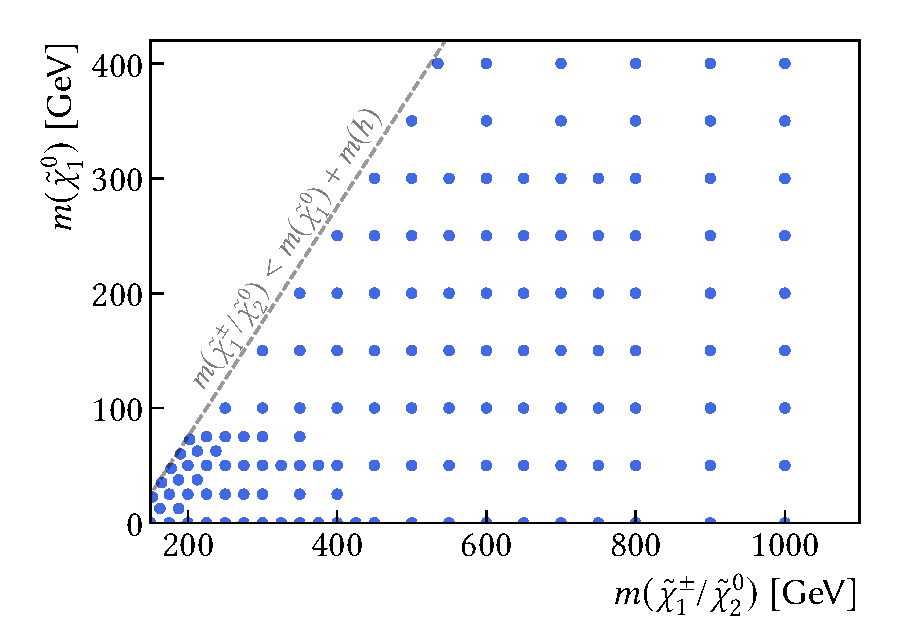
\includegraphics[width=0.5\textwidth]{signalgrid}}
%\end{figure}

In searches for \gls{bsm} physics at the \gls{lhc}, it is common to use simplified models~\cite{SimplifiedModels1:2008ag,SimplifiedModels2:2011wf,Alves:2011sq} as a way of reducing the available parameter space to a manageable level.
%Simplified models do not aim to represent complete supersymmetric models but are mostly defined by the empirical objects and kinematic variables used in the searches, typically allowing only a small number of sparticles to be involved in the decay chain (usually only two or three).
Simplified models do not aim to represent complete supersymmetric models but are mostly defined by a single (or a few selected) decay chain(s) allowing only a small number of participating sparticles, usually only two or three.
Other sparticles are decoupled by setting their masses to be kinematically inaccessible at current collider experiments. The decay chains of the participating sparticles are determined by fixed branching ratios, often set to be 100\%.
Experimental bounds from non-observation of a given model are then typically presented in function of the physical masses of the sparticles involved in the decay chain.
The model space spanned by the free parameters of the simplified model is typically called a \textit{signal grid}, as each set of distinct mass parameter values, called \textit{signal point}, occupies a single discrete point in this space. \Cref{fig:signalgrid} illustrates the signal grid used in \cref{part:simplified_model_analysis} of this thesis. The exact details of the signal grid are further discussed in \cref{sec:models_used}.
 
Simplified models have the inherent advantage that they circumvent the issue of having to search for \gls{susy} in a vast parameter space where many of the parameters may only have small effects on observables. Their interpretation in terms of limits on individual \gls{susy} production and decay topologies in function of sparticle masses is straightforward and very convenient.
The hope is, that simplified models are a reasonable approximation of sizeable regions of parameter space of the more complete model they are embedded in~\cite{pdg2020}. The obvious downside is, however, that the limits obtained in simplified models are not automatically a good approximation of the true underlying constraint on the respective model parameter when interpreted in more complete \gls{susy} models.
Often, the constraints set on sparticle masses in simplified models, significantly overestimate the true constraints obtained in more complex \gls{susy} spectra, especially when the usually assumed 100\% branching fractions are no longer realised in more complete models (see \eg~\cite{Ambrogi:2017lov,Buchmueller:2013exa}).

\begin{figure}
\floatbox[{\capbeside\thisfloatsetup{capbesideposition={right,center},capbesidewidth=0.45\textwidth}}]{figure}[\FBwidth]
{\caption{Cross sections of different \gls{susy} production processes at $\sqrt{s}=\SI{13}{\TeV}$ in $pp$ collisions. Cross sections for pair production of electroweakinos are significantly smaller than, \eg, those for pair production of gluinos. The shaded bands correspond to the theory uncertainty of each cross section. Cross sections taken for coloured and electroweak sector taken from \references\cite{Beenakker:2016lwe,Beneke:2009ye} and \references\cite{Fiaschi:2018hgm,Fuks:2012qx,Fiaschi:2018xdm}, respectively.}\label{fig:SUSY_xsecs}}
{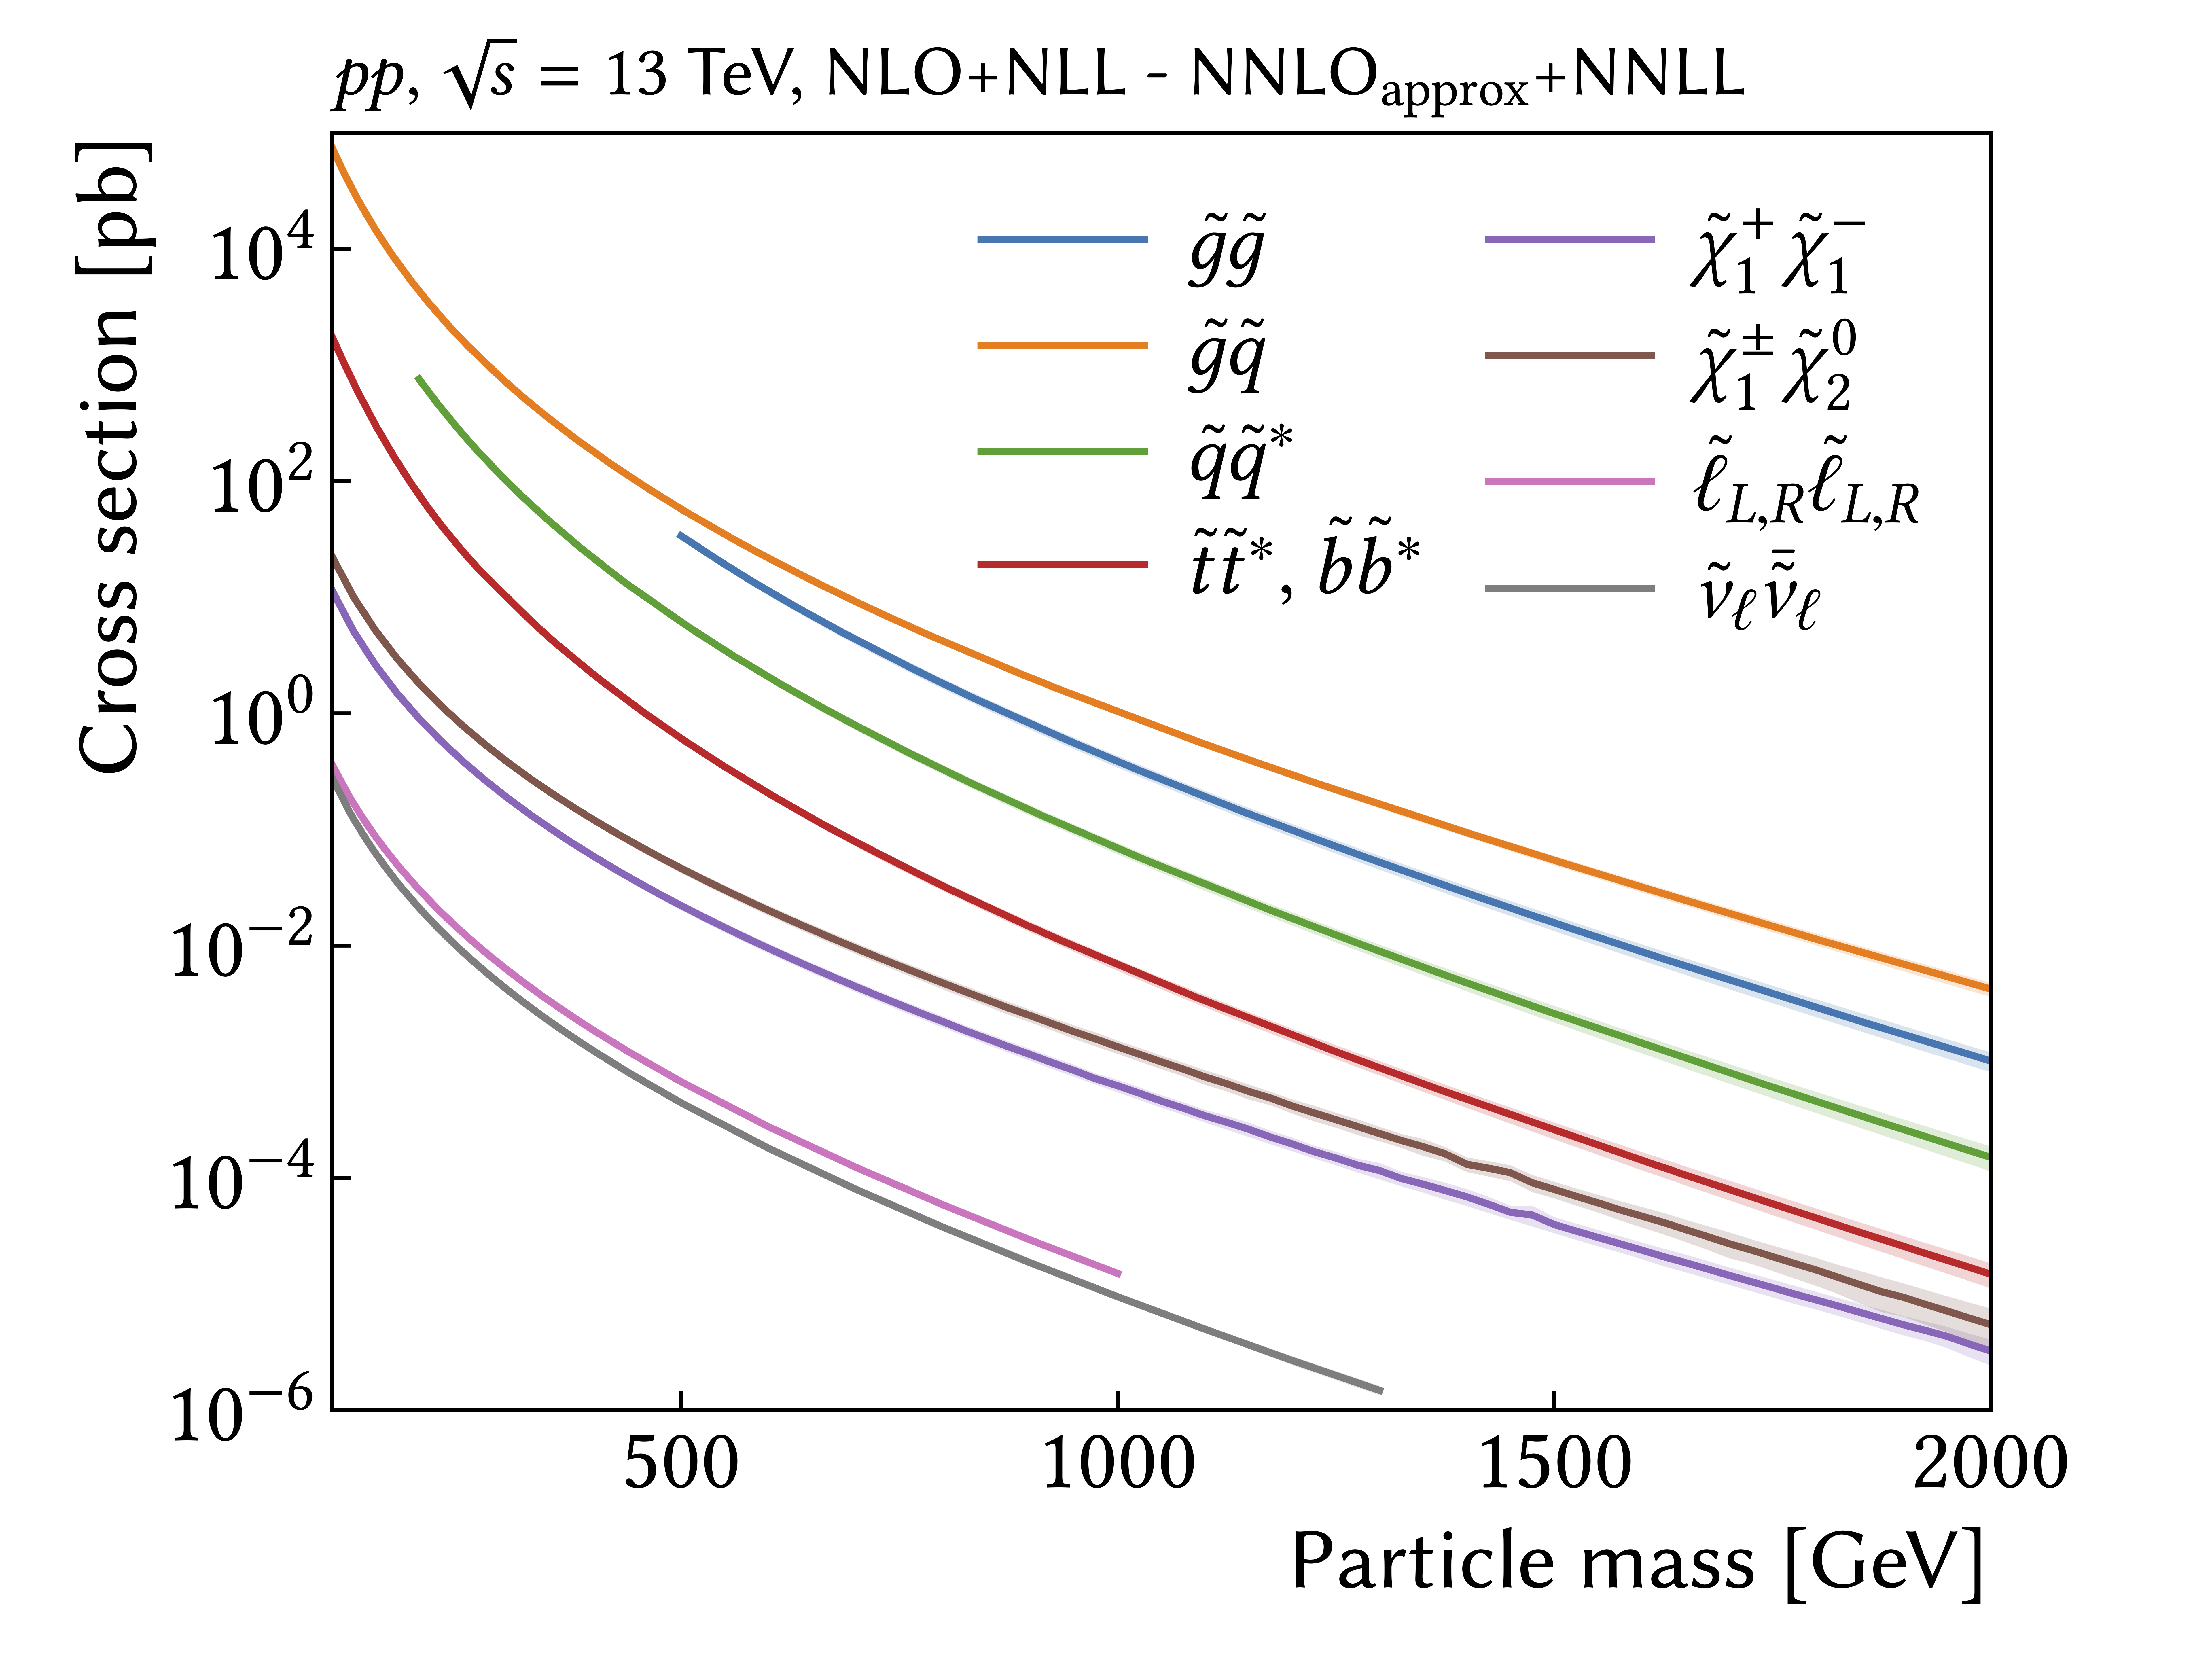
\includegraphics[width=0.5\textwidth]{SUSY_xsecs}}
\end{figure}

One way of circumventing these issues, while sticking to the simplified model approach, is to ensure that the limits obtained in different simplified models involving different production and decay mechanisms are combined into limits representing more complex \gls{susy} spectra.
In such an approach, the simplified model limits can be seen as building blocks for more realistic \gls{susy} models that include many different production processes and decay modes.
Another possibility is to perform reinterpretations of \gls{susy} searches---optimised for one ore more such simplified models---in more complete (and high-dimensional) \gls{susy} model spaces, like \eg, in the \gls{pmssm}. This cannot only demonstrate the sensitivity of existing \gls{susy} searches beyond simplified models, but also potentially identify blind spots and model regions not covered by current searches.
In addition, connections to (in)direct \gls{dm} searches and various \gls{sm} measurements can be explored this way. Recent efforts in this direction include, \eg, \references\cite{Ambrogi:2017lov, Aaboud:2016wna, pMSSM-scan-run1:2015baa}. As will be discussed in \cref{part:reinterpretation} of this thesis, efforts reinterpreting ATLAS searches for \gls{susy} in the \gls{pmssm} are currently ongoing. In \cref{ch:pmssm}, a reinterpretation of the search for electroweakinos presented herein using a set of \gls{pmssm} models, is discussed.


\section{Search for electroweakinos}

\begin{figure}
	\centering
	\begin{subfigure}[b]{0.33\linewidth}
		\centering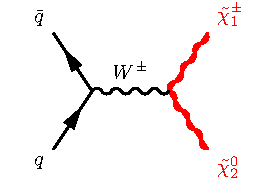
\includegraphics[width=.9\textwidth]{electroweakino_production_1}
		\caption{\label{fig:electroweakino_production_1}}
	\end{subfigure}%
	\begin{subfigure}[b]{0.33\linewidth}
		\centering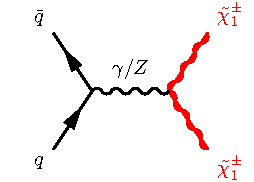
\includegraphics[width=.9\textwidth]{electroweakino_production_2}
		\caption{\label{fig:electroweakino_production_2}}
	\end{subfigure}%
	\begin{subfigure}[b]{0.33\linewidth}
		\centering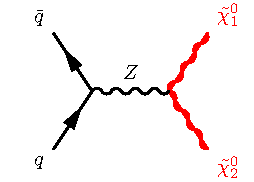
\includegraphics[width=.9\textwidth]{electroweakino_production_3}
		\caption{\label{fig:electroweakino_production_3}}
	\end{subfigure}	
	\caption{Dominant diagrams for production of electroweakino pairs at the Large Hadron Collider. Adapted from \reference\cite{Martin:1997ns}.}\label{fig:electroweakino_production}
\end{figure}

While both the ATLAS experiment~\cite{ATL-PHYS-PUB-2021-007} and CMS experiment~\cite{CMSsummary} at the \gls{lhc} at CERN set strong limits on the presence of gluinos and squarks at the TeV scale, the limits on electroweakinos are mostly still below $\SI{1}{\TeV}$. 
The reason for the relatively low limits on electroweakinos are the low cross-sections of electroweakino production, compared to those of squark and gluino production.
As can be seen in \cref{fig:SUSY_xsecs}, the cross sections for $\charg\neutr$ pair production (the main production process considered in the following) is more than two orders of magnitude smaller than that for gluino pair production.  

Apart from the electroweakino mass limits set by the current collider experiments, some additional limits from the LEP experiments are still relevant in some corners of the phase space. Combining the results from all four LEP experiments leads to a general lower chargino mass limit of $\SI{103.5}{\GeV}$, except for scenarios with a low sneutrino mass~\cite{lep_susy_results}. For small mass splittings between the chargino and the \gls{lsp}, the lower limit is a little weaker, with dedicated searches excluding charginos with $m(\charg) < \SI{91.9}{\GeV}$~\cite{lep_susy_results}. For mass splittings larger than $\SI{1.5}{\GeV}$ and up to $\SI{50}{\GeV}$, the \gls{lep} chargino limits have recently been superseded by a dedicated ATLAS search for compressed \gls{susy} scenarios~\cite{SUSY-2018-16}, excluding chargino masses up to $\SI{240}{\GeV}$ for a mass splitting of $\SI{7}{\GeV}$. For the neutralino, a lower limit on the lightest neutralino mass comes from limits on the invisible width of the $Z$ boson, excluding $m(\lsp) < \SI{45.5}{\GeV}$, depending on the $Z$--neutralino coupling~\cite{pdg2020}.

\subsection{Production of electroweakinos at the Large Hadron Collider}

If gluinos and squarks are heavier than a few TeV, \ie too heavy to be within reach of the \gls{lhc}, the direct production of electroweakinos might be the dominant production mode of SUSY. At hadron colliders, electroweakinos can be pair-produced directly via electroweak processes. The direct production of electroweakino pairs dominantly happens through electroweak gauge bosons from \textit{s}-channel $q\bar{q}$ annihilation, as shown in \cref{fig:electroweakino_production}. Contributions from \textit{t}-channels via squark exchange are typically of less importance~\cite{Martin:1997ns}.


\subsection{Models used within this work}\label{sec:models_used}

%\begin{figure}
%	\centering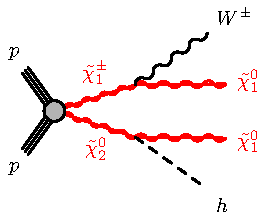
\includegraphics[width=.4\textwidth]{C1N2-WhN1N1}
%	\caption{Diagram for $\charg\neutr$ pair production with subsequent decays into $\charg\rightarrow W^\pm\lsp$ and $\neutr\rightarrow h\lsp$.}\label{fig:Wh_model}
%\end{figure}

\begin{figure}
	\centering
	\begin{subfigure}[b]{0.45\linewidth}
		\centering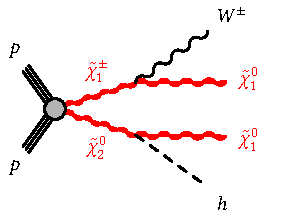
\includegraphics[width=.85\textwidth]{c1n2_wh}		
		\vspace{1em}
		\caption{\label{fig:Wh_model}}
	\end{subfigure}\hfill
	\begin{subfigure}[b]{0.55\linewidth}
		\centering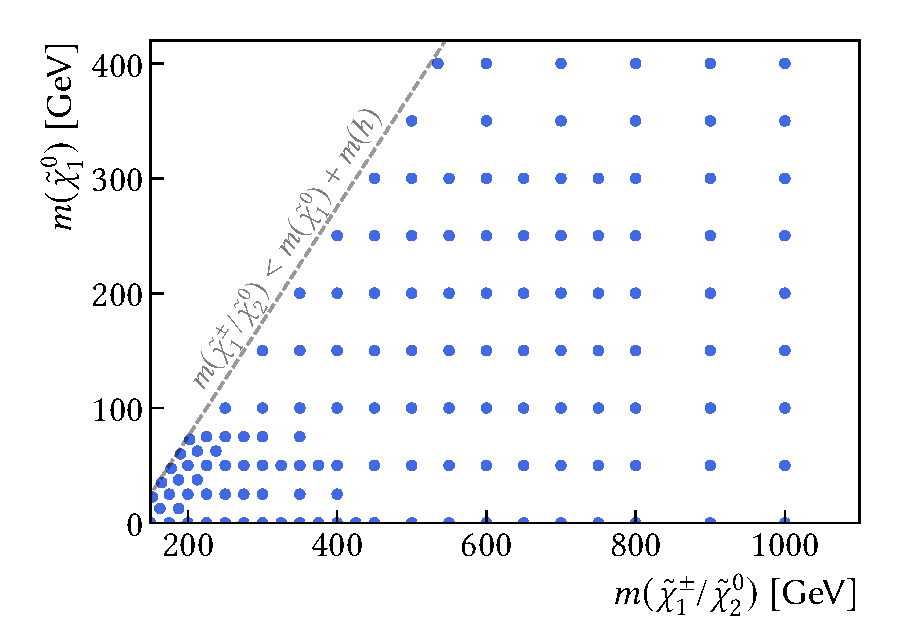
\includegraphics[width=.9\textwidth]{signalgrid}
		\caption{\label{fig:signalgrid}}
	\end{subfigure}	
	\caption{Simplified model used in this thesis. Fig.~\subref{fig:Wh_model} shows a diagram for $\charg\neutr$ pair production with subsequent decays into $\charg\rightarrow W^\pm\lsp$ and $\neutr\rightarrow h\lsp$. Fig.~\subref{fig:signalgrid} shows the signal grid used. Each discrete point represents a different signal model with a unique set of $\charg$/$\neutr$ and $\lsp$ mass parameters.}\label{fig:models_used}
\end{figure}

%\begin{figure}
%\floatbox[{\capbeside\thisfloatsetup{capbesideposition={right,center},capbesidewidth=0.4\textwidth}}]{figure}[\FBwidth]
%{\caption{Diagram for $\charg\neutr$ pair production with subsequent decays into $\charg\rightarrow W^\pm\lsp$ and $\neutr\rightarrow h\lsp$.}\label{fig:Wh_model}}
%{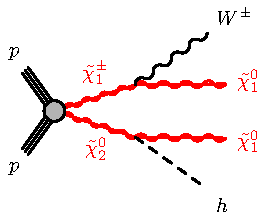
\includegraphics[width=0.5\textwidth]{C1N2-WhN1N1}}
%\end{figure}

In \gls{susy} scenarios where the sleptons and charged and pseudoscalar Higgs bosons are heavier than the charginos and neutralinos, a relatively pure wino lightest chargino decays predominantly through $\charg\rightarrow W^\pm\lsp$, while the next-to-lightest neutralino decays via $\neutr\rightarrow Z/h\lsp$. If, in addition, the higgsinos are much heavier than the wino, and the mass splitting between the two lightest neutralinos is larger than the Higgs boson mass, the decay $\neutr\rightarrow h\lsp$ can be the dominant decay mode of the $\neutr$. In this case, both the $\charg$ and $\neutr$ are wino-like and nearly mass-degenerate.

The main model used in the following is a simplified model considering direct production of a $\charg\neutr$ pair, where the lightest chargino decays via $\charg\rightarrow W^\pm\lsp$ and the next-to-lightest neutralino decays via $\neutr\rightarrow h\lsp$, each with 100\% branching ratio.
The lightest chargino $\charg$ and the next-to-lightest neutralino $\neutr$ are assumed to be degenerate in mass and pure wino states, while the lightest neutralino $\lsp$ is considered to be a pure bino \gls{lsp}.
The mass parameter hierarchy for this model is thus \mbox{$\vert M_1 \vert < \vert M_2 \vert \ll \vert\mu\vert$}. 

The $\charg$/$\neutr$ and $\lsp$ masses are free parameters that are systematically varied, creating a two-dimensional signal grid to be scanned and compared to data. \Cref{fig:signalgrid} shows the two-dimensional signal grid used in \cref{part:simplified_model_analysis} of this thesis. In the simplified model, the Higgs boson mass is set to $\SI{125}{\GeV}$ in accordance with the measured value~\cite{HIGG-2012-27,CMS-HIG-12-028} and its branching ratios are the ones from the \gls{sm}. A diagram for the simplified model considered is shown in \cref{fig:Wh_model}.

In addition to the simplified model targeted by the \gls{susy} search presented in the following, an additional class of models is considered in the second part of this work. These models are sampled directly from the \gls{pmssm} parameter space and are used to reinterpret the aforementioned search for direct pair production of electroweakinos. The mass spectrum of a representative \gls{pmssm} model point used is shown in \cref{fig:slha_example}. Additional details on the sampling and phenomenology of the \gls{pmssm} models are given in~\cref{ch:pmssm}. 


\begin{figure}
	\centering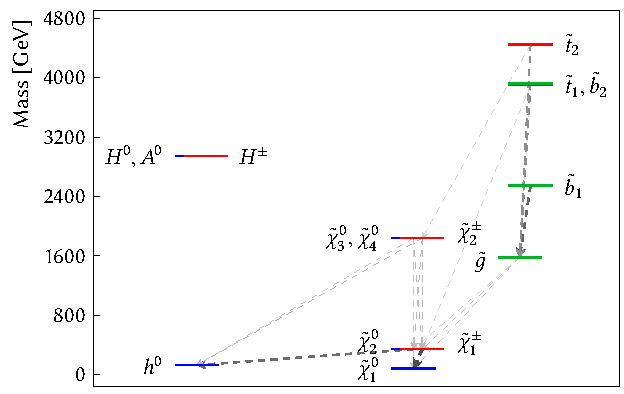
\includegraphics[width=.6\textwidth]{thesis_plot_9127}
	\caption{
Mass spectrum of an representative \gls{pmssm} model. The branching fractions of the different decays are indicated through the width and and greyscale colour (black being 100\%, white being 0\%) of the arrows. Branching fractions smaller than 10\% are suppressed for the sake of visibility. Figure generated using \texttt{pyslha}~\cite{pyslha:2013jua}.}
\label{fig:slha_example}
\end{figure}

%\begin{figure}
%\floatbox[{\capbeside\thisfloatsetup{capbesideposition={right,center},capbesidewidth=0.4\textwidth}}]{figure}[\FBwidth]
%{\caption{Diagram for $\charg\neutr$ pair production with subsequent decays into $\charg\rightarrow W^\pm\lsp$ and $\neutr\rightarrow h\lsp$.}\label{fig:slha}}
%{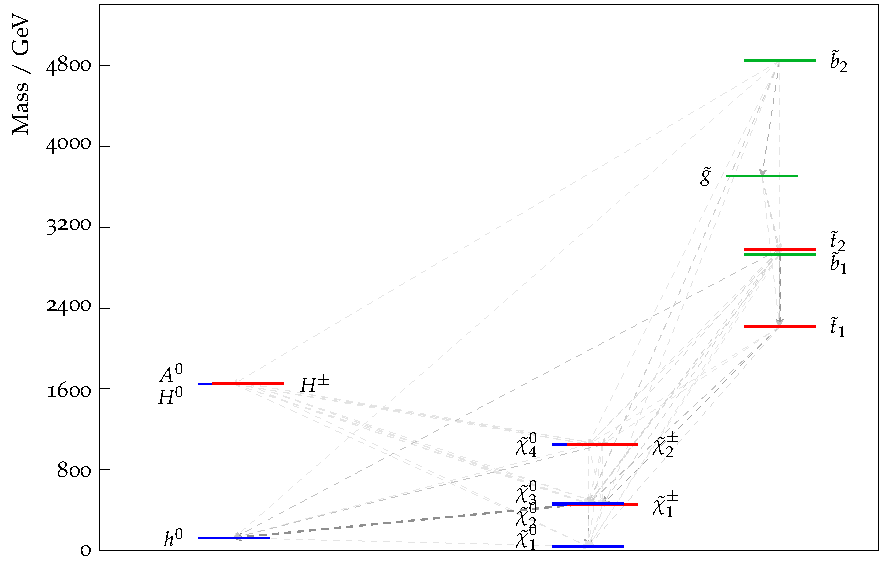
\includegraphics[width=0.5\textwidth]{slha}}
%\end{figure}



